\documentclass{article}

%Document Information
\title{GCE Computer Science Component 3}
\author{Edward Robert Karol Demkowicz-Duffy}

%Define page margins with geometry
\usepackage[a4paper, total={6.25in, 9in}]{geometry}

%Remove footnote ruling
\renewcommand*\footnoterule{}

%Import package for forcing image locations
\usepackage{float}

%Import package for images and set graphics path to /images
\usepackage{graphicx}
\graphicspath{{./images/}}

%Import package for managing sections, configure to add a new page every section
\usepackage{titlesec}
\newcommand{\sectionbreak}{\clearpage}
\newcommand{\subsectionbreak}{\clearpage}

%Import package for handling enumeration and configure it
\usepackage{enumitem}
\setlist[description]{leftmargin=\parindent,labelindent=\parindent}

%Import package for code
\usepackage{listings}
\lstset{defaultdialect=[Sharp]C}
\usepackage{xcolor}
%Configure code syntax highlighting
\definecolor{codenormal}{rgb}{0.862, 0.862, 0.862}
\definecolor{codekeyword}{rgb}{0.337, 0.603, 0.839}
\definecolor{codecomment}{rgb}{0.341, 0.650, 0.290}
\definecolor{codestring}{rgb}{0.839, 0.615, 0.521}
\definecolor{backcolour}{rgb}{0.117, 0.117, 0.117}
%Define pseudocode
\lstdefinelanguage{psuedocode}
{
  %Keywords
  morekeywords={
      global,
      str,
      int,
      float,
      list,
      print,
      input,
      for,
      to,
      next,
      do,
      until,
      AND,
      OR,
      NOT,
      if,
      then,
      elseif,
      endif,
      switch,
      case,
      default,
      endswitch,
      function,
      return,
      endfunction,
      procedure,
      endprocedure,
      array
  },
  sensitive=true, % keywords are not case-sensitive
  morecomment=[l]{//}, % l is for line comment
  morecomment=[s]{/*}{*/}, % s is for start and end delimiter
  morestring=[b]" % defines that strings are enclosed in double quotes
}
%Define style
\lstdefinestyle{mystyle}{
    backgroundcolor=\color{backcolour},
    commentstyle=\color{codecomment},
    keywordstyle=\color{codekeyword},
    stringstyle=\color{codestring},
    basicstyle=\footnotesize\color{codenormal}\linespread{1.15},
    numberstyle=\color{black},
    breakatwhitespace=false,
    breaklines=true,
    captionpos=b,
    keepspaces=true,
    numbers=left,
    numbersep=5pt,
    showspaces=false,
    showstringspaces=false,
    showtabs=false,
    tabsize=2
}
%Apply style
\lstset{style=mystyle}

%Import package for drawing flowcharts
\usepackage{tikz}
\usetikzlibrary{shapes.geometric, arrows}
%Define styles for the flowcharts
\tikzstyle{startstop} = [rectangle, rounded corners, minimum width=3cm, minimum height=1.5cm,text centered, text width=4cm, draw=black, fill=red!30]
\tikzstyle{io} = [trapezium, trapezium left angle=70, trapezium right angle=110, minimum width=3cm, minimum height=1.5cm, text centered, text width=4cm, draw=black, fill=blue!30]
\tikzstyle{process} = [rectangle, minimum width=3cm, minimum height=1.5cm, text centered, text width=4cm, draw=black, fill=orange!30]
\tikzstyle{decision} = [diamond, minimum width=3cm, minimum height=1cm, text centered, text width=4cm, draw=black, fill=green!30]
\tikzstyle{arrow} = [thick,->,>=stealth]

\begin{document}
    \pagenumbering{gobble}
    \maketitle
    
    \tableofcontents
    \pagenumbering{arabic}
    
    %Set the table of contents depth to only show sections and subsections
    \addtocontents{toc}{\setcounter{tocdepth}{2}}
    \section{Analysis}
    \subsection{Problem Description}
    \paragraph{•}
    My client is a personal friend and the owner of a business that is based around the sale of novelty clocks and coasters manufactured from or based on vinyl records. 
    They buy (often) second hand vinyl records from various sources, cut out the album art in the middle and use that to mount a clock mechanism on, then package it in it’s original sleeve modified to become a box as a clock to be hung or place on a surface. 
    They also manufacture sets of coasters which are artificially manufactured to appear as vinyl records, sold in sets of matching bands or contemporary albums. 
    Their present sales solution is in three parts:
    \begin{itemize}
    \item Online sales through third party storefronts Etsy and eBay
    \item Face-to-face sales at the client’s stall at the regular Manchester Christmas markets
    \item Other face-to-face sales at any other events the client or their employees may wish to attend, irregularly
    \end{itemize}
    This solution is inconvenient for multiple reasons. 
    The two storefronts provide quite different experiences and tools for people wanting to sell their products on their platforms and thus my client often finds it difficult to deduce trends and critical values like net profits in their overall online sales. 
    Sales at the Christmas markets are difficult to keep track of as the square they are held in get crowded and the client/their employees frequently lose track of sales, which can be found at the end of the day by examining existing records, money gained and remaining stock; but is still an obstacle to clear analysis of the client’s sales. 
    Stalls at other events are usually set up at short notice, and similar logistical problems tend to arise as with the Christmas markets, but with less pre planning time and available information they also tend to be more difficult to solve. 
    \paragraph{•}
    The client would like a web app which provides a quality sales experience to customers, and powerful management tools and information for employees. 
    It must have an online storefront, a (modifiable) storage method to track products and all their related information (most importantly stock and price) and sales of said products. 
    Users should have to register to make purchases. 
    Employees should be to view and modify products. 
    There should be easy tools that specialize in managing stock and sales both at the beginning and the end of a day when the client sells their products at an event, be it unexpected or scheduled. 
    The client also specifically requests that employees be able to view statistics and basic analysis of sales displayed in an easy-to-understand way. 
    Employees with special permission should also be able to modify the accounts of both customers and other employees and delete or add products to the program’s storage. 
    Furthermore, the website must be secure, with both customers’ and employees’ data appropriately protected and must appear professional and easy to comprehend.
    
    \subsection{Stakeholders}
    \paragraph{•}
    Stakeholders are identified here as being people who must use, or will be directly affected by, the program. 
    There are three primary stakeholders, who must be born in mind during the creation of the web app:
    \paragraph{Customers}
    These are the most important stakeholders as they as the client’s source of income. 
    They must have the easiest and most convenient experience possible, to retain their attention on the products the client wishes to sell to them. 
    They will benefit from the project by having a quick and easy way to exchange money for goods they wish to buy. 
    As such, the interface they use should be carefully and logically laid out, with no unneeded features or artefacts on it. 
    Products should be described clearly and concisely so the customers know exactly what they are buying and all other information relevant to it.
    \paragraph{Staff}
    These are the people employed by the client who manage their stock and make sales in person. 
    Their side of the web app will be used for swift and easy viewing of stock and statistics – they may also need to modify stock data. 
    Therefore it must provide the quickest and most powerful ways to manage current stock and sales at physical stalls, and helpful processed sales data.
    \paragraph{Administrators} 
    These are senior employees who have all the responsibilities of other employees but have more power over the company’s assets. 
    They have the same requirements as regular employees, but also need to be able to view the data of customers and ordinary employees, be able to add whole new products to the set (and delete existing ones), be able to change the passwords of and delete accounts (be they employee or customer) and be able to view technical data like logs.
    
    \subsection{Solving with Computational Methods}
    \paragraph{•}
    The client requires a centralised service for distributing their products en masse to customers who may be international – a website or web app is perfect for this purpose as it can be accessed anywhere, can be easily translated, and requires little to no uncommon knowledge to use and access. 
    It can be accessed from many places at once and run in parallel in all these places without compromising at all in any.
    \paragraph{•}
    The client requires a service that will supply their company with processed data that will help them analyse their sales strategies and improve them. 
    Computers excel at this as it is a repetitive numerical task which can be completed by a processor much faster than a human analyst. 
    In addition to this, computers can scale easily to very large amounts of data, whereas other methods (aforementioned analyst) would likely struggle to cope in comparison.
    \paragraph{•}
    The client requires a method for organising all their stock in a central location, with the ability for it to be accessed and changed from anywhere at any time. 
    An always-on, internet-connected data source is an exceptional solution for this problem because besides matching all the required criteria since it can be accessed from anywhere by anyone with the appropriate credentials, it can add useful functionality to them by logging all information transfers and enforcing logical rules like relationships between data and correct formatting. 
    The same data source can store information about both the customers and employees who use it for increased availability of data. 
    This ties in with the previous requirement as all the data needing to be processed being stored in one (digital) location is extremely helpful for any computerised process trying to access it, keeping time taken to do that processing short.
    \paragraph{•}
    Another advantage of the service being hosted online is that issues that may arise with the software are quick and easy to patch out as the patch can be deployed immediately to the only host with little to no downtime, meaning the service remains almost completely uninterrupted.
    
    \subsection{Research}
    \subsubsection{The Client's Current Solution}
    \paragraph{•}
    As mentioned in the problem description, the client employs eBay and Etsy to sell their products online; however as I have covered these examples below I will focus on the physical sales element in this section.
    \paragraph{Advantages}
    There are several advantages to this method of selling, most of which are related to the fact that the customer can talk to an employee in person and that they can view the product they wish to buy first hand.
    \paragraph{•}
    The customer can examine the product on site, and view properties of it that they may not be able to judge through a website like size, weight and "true" colour.
    This increases the probability that the customer will make a purchase considerably, and so would be desirable to try to compensate for in the we application - the methods this could be accomplished through are essentially to ensure the product is represented on it's "page" as accurately and fully as possible.
    Dimensions should be included along with multiple images of the product from different angles and in different lighting conditions.
    \paragraph{•}
    The customer can also talk to the employee for an extended period of time if they wish, which gives the employee the opportunity to convince them to purchase the product and to further enhance their image in the eyes of the customer (i.e. beyond what the customer has viewed of the array of products and the stall itself).
    Again, it is hard to provide a comparable service on a website to this.
    One solution would be to include a live text chat interface on the web application.
    This would require constant employee presence which is not feasible for my client as their company is not large enough or well-known enough to warrant having a team of support staff available.
    Another method would be to provide a phone number on the website and encourage people to call it if they have enquiries so as to reduce the requirements on the hosting machine and potentially the number of people needed to answer, but this would still suffer from the same problems as the first proposal (albeit less so).
    \paragraph{Disadvantages}
    Employees can only bring and display so much stock to a physical event, which means the choice and availability customers see is severely stunted.
    A web application would inherently solve this issue because the entire inventory is displayed simultaneously so this does not need to be considered.
    \paragraph{•}
    Furthermore, the inventory the client takes with them is vulnerable to theft and damage while it is on display at the event.
    This is another problem that is solved by developing a web application as a replacement because no stock is "exposed" until it has been sold to a customer.
    \subsubsection{Existing Successful Examples}
    \paragraph{•}
    This type of software is commonly used in ordinary life today.
    Multiple excellent examples already exist, some of which the client already utilizes.
    Three prominent extremely successful public examples are listed below:
    \begin{itemize}
    \item Amazon
    \item eBay
    \item Etsy
    \end{itemize}
    \paragraph{Amazon}
    This site is an enormous online marketplace which allows any verified entity to buy or sell goods there.
    It features extensive methods for displaying information about the goods listed on it, including images, hand written descriptions, multiple variants, stock amounts, delivery information (cost, areas available to deliver to) and in depth public user reviews.
    It also contains algorithms designed to promote other products to the user, displayed in the form of recommendations, usually labelled "people who bought this bought" or other such categories.
    I would guess that these are generated from the logged-in user's purchase history and viewing history by categorising all products on the website, then suggesting the most popular products in the categories the user views and purchases from the most.
    This is an excellent method to retain user attention and encourage users to stay on the site and spend more money.
    The feature would be excellent to incorporate into my own application, however it could prove algorithmically quite complex to implement.
    \paragraph{•}
    The site allows users to store payment information and delivery addresses for ease of use in future transactions - another great way to make user's experience much easier and quicker, which will in turn increase the chances of them making more purchases on the site.
    The site stores customer's order history in depth with information pertaining to when they were ordered, how much was paid, when they were delivered and even who to.
    In addition, they provide live tracking of orders which are in the process of being delivered.
    \paragraph{•}
    Amazon also displays advertisements for currently running sales, new products and even new features.
    This draws the attention of users to popular products which they are more likely to buy.
    More so, the efficiency of shopping (i.e. the amount of time it takes to locate a specific product) is much improved by a large array of searching, sorting and filtering options when browsing available goods.
    Users can sort by price, name and search relevance to name but a few, and can search product names across the whole site or within specified categories.
    
    \paragraph{eBay}
    This is a site similar to Amazon which allows buyers and sellers to make transactions in exchange for goods and services online.
    In contrast to Amazon, however, eBay facilitates time-limited auctions to be hosted which buyers can place bids on during a set time period, where the product will be sold to the highest bidder who will pay their named price to the seller.
    The user interface surrounding this feature is designed fantastically to make it as simple and easy as possible for customers to place bids - it shows them the starting price, the time remaining (live) and the current highest bid.
    It makes placing a bid as easy as entering a value in a text box and pressing a button with extremely low latency, so that competitive bidding can occur fairly towards the end of the time period which I frequently observed to drive the final price much higher within a small time frame.
    This means sellers can create highly competitive environments for optimum profit, something I thought my client would appreciate greatly, but upon contacting them they informed me they were not interested in auctioning their products.
    Still, there are definitely notes to be taken here as the design philosophies of the highly intuitive GUI displayed on the auction page can be applied well to the selling pages of my own project.
    \\
    eBay offers many of the features Amazon does, namely the recommendations of other products, all the delivery related features and the saving of information related to those deliveries (addresses and payment methods).
    \paragraph{Etsy}
    This is another online marketplace with a similar goal to the aforementioned two.
    It's distinguishing feature is that it allows sellers to design and construct their own personalised pages to display their products and their information, referred to as their "shop".
    This is a powerful function as it allows sellers to present themselves as they wish to prospective buyers, be it using particular colour palettes or shape designs, this sets the "attitude" of the seller and creates a "mood" relating to them.
    While this feature on it's own is not especially relevant to my client's needs as they wan to sell only as one entity in their own location, the core concept of presenting an impression to the user is a powerful way to get a consistent "feel" across the site which fits with my client's intended public image.
    \subsubsection{Conclusion}
    Key features shared by all the successful examples are:
    \begin{itemize}
    \item Algorithmically-generated recommendations for the customer based on their order and viewing history.
    While a full implementation of this may prove to be out of the scope of my project, it is clearly a useful feature to implement that may well increase the chance of purchases being made by users.
    Alternatives could be to show users "buy it again" or "next in the set" options.
    \item Convenience-based features.
    All the websites I examined were obviously designed to make the user experience as slick as possible.
    This is very helpful for the seller and website because it encourages the user to spend more time browsing and buying due to the whole process being easier.
    As such, it should be an important success criterion that the user experience is as "smooth" as possible to promote the most time spent on the website.
    \item Comprehensive searching and filtering tools.
    These are designed to assist customers finding the product that suits their needs.
    The products which will be displayed on my project will be more similar than those present on the websites examined, but the idea of searching through them can be carried over still.
    The web app I will build should offer similar functionality if it wants users to locate products as swiftly as possible.
    \item Information-laden lists of products.
    These worked exceptionally well when used in conjunction with the above tools.
    Each product is represented in short with crucial information clearly available in a small space, which further assists in finding the desired products.
    \item Plentiful information related to the item the user is viewing.
    Each website has an individual page for each item the user views containing a plethora of data that they may want to find about the product.
    All three website showed a "slide show" of photographs or other images of the product they were viewing, and allowed them to zoom in and examine them.
    Descriptions written by the sellers featured markdown formatting to allow text effects such as bolding, italics, links and underlining which help express information the seller writes more effectively and strikingly.
    Stock and prices are shown in depth, with exact numbers of stock left and the delivery costs displayed clearly and prominently in the foreground of the page's design.
    These would all be good ideas to follow from.
    \item Storage and easy access of the user's data.
    This includes past payments and addresses so the user doesn't have to go and retrieve their cards when making a purchase, which in turn keeps them browsing longer and improves their experience making transactions.
    The sites also store all a user's past orders and display them in a concise way upon request, with money spent, which product, the amount of that product and the date the order was placed all very visible.
    This is a feature which I can and plan to implement in my own website very effectively, as I already planned to store extended data about any orders made within the program.
    \end{itemize}
    Appearance appears to play a key role in usability too - all the websites I examined had consistent colour palettes and designs across all pages which gave a distinct impression of professionalism.
    \subsubsection{Laws}
    There are several laws pertaining to data hosted online.
    Since the service I intend to construct will store sensitive personal information, the Data Protection Act 1998 dictates that the service provider is responsible for any damage or theft of that data.
    My solution must be secure enough that the client can be confident their user's data is safe from people who shouldn't see it as they would be held liable should it be stolen.
    \subsection{Software and Hardware Requirements}
    \paragraph{•}
    As this software will be interacted with in different ways to how it is run at it’s actual location, I have included two sets of hardware requirements; one for the end user (be they employee or customer) and one for the server hosting the software:
    
    \subsubsection{Client Computers}
    \begin{itemize}
    \item The latest version of a modern browser. 
    I recommend Google Chrome, Microsoft Edge, Mozilla Firefox, Opera or Safari.
    \item A computer which can run that browser. For reference, I have taken the requirements\footnote{https://www.mozilla.org/en-US/firefox/58.0.2/system-requirements/} for Mozilla Firefox, which is regarded as an industry standard:
    \begin{itemize}
    \item Pentium 4 or newer processor that supports SSE2
    \item 512MB of RAM / 2GB of RAM for the 64-bit 
    \item 200MB of hard drive space
    \end{itemize}
    \item An internet connection with download speed equal to or exceeding 5MB/s (megabits per second)
    \end{itemize}
    
    \subsubsection{Host Computer}
    \begin{itemize}
    \item At least 5GB of available secondary storage with a high read/write rate
    \item A modern high-performance server processor with 4 or more cores clocked at more than 3GHz
    \item At least 16GB of RAM
    \item An internet connection with download and upload speeds equal to or exceeding 1GB/s (gigabits per second)
    \end{itemize}
    
    \subsection{Success Criteria}
    \begin{enumerate}
    \item Write a web application that holds information about orders, customers, products and employees. 
    \item The web application must show users the appropriate data for their role in using the program; products data to customers, managerial data to employees, all data to administrators.
    \item The web application must allow customers to create their own credential combinations which they must use to identify themselves when interacting with the web application.
    \item The web application must allow customers to select products they would like to buy and purchase them. 
    Furthermore, it must provide them adequate data to make this decision on. 
    \item The web application must allow employees to view and edit information stored in the application which they are permitted to. They may view:
    \begin{itemize}
    \item All data related to all products
    \item All data related to placed orders
    \item The usernames of all registered customers
    \end{itemize}
    They may edit: 
    \begin{itemize}
    \item The stock value of all products
    \item The passwords of registered customers
    \end{itemize}
    \item The web application must allow administrators to view and edit information stored in the application which is likely to be necessary. They may view:
    \begin{itemize}
    \item All data related to all products
    \item All data related to placed orders
    \item The usernames and personal data of all registered customers
    \item The usernames and personal data of all registered employees
    \item The background logs kept by the application
    \end{itemize}
    They may add:
    \begin{itemize}
    \item Employee accounts
    \item Products
    \end{itemize}
    They may delete:
    \begin{itemize}
    \item Customer accounts
    \item Employee accounts
    \item Products
    \end{itemize}
    \item The web application should show employees helpful data on sales, including but not limited to:
    \begin{itemize}
    \item Sales per week
    \item Sales per month
    \item Sales per year
    \item Sales per customer
    \end{itemize}
    It should also be able to show not just sales volume but total income for all of the above. It should display these data in a graphical visualisation which allows quick and easy interpretation of the data.
    \item The web application should provide a facility for helping employees manage sales in person.
    This facility should be able to track what products the employee has taken with them and "reserve" them from the main inventory.
    It should be able to record what was sold at the end of the event as specially marked orders, and return all unsold "reserved" items to the main inventory.
    \item All the above should be accomplished such that it is hard enough for outside hostile elements to access sensitive data to allow the client to be confident that the service won't breach the Data Protection Act 1998.
    \end{enumerate}
    
    \section{Design}
    \subsection{Problem Decomposition}
    \paragraph{•}
    This problem must be approached with computation in mind if I am to succeed.
    \paragraph{•}
    I will begin by abstractifying the components of the problem while sticking to my success criteria to keep my goals in sight.
    For this I should focus on compartmentalising the key individual challenges of the project, i.e. login system, data storage method e.t.c.
    As I do this, I will record a plan of the project either on paper or digitally which lays out the requirements of each section and the implementation methods I intend to use.
    The plan should include a list of pages and background processes that the application needs to run.
    \paragraph{•}
    Once I firmly believe my plan is suitable to the problem, I will begin to think about the appearance of the web application.
    I will prototype several sketches for the different pages that I think are appropriate, consult the client with them, use their feedback to improve some of them and show the client again.
    I can repeat this process until we reach a prototype me and the client are both satisfied with.
    When I have a final prototype, I will experiment with different core rules for all pages to follow based on that prototype - these is important because it retains a consistent look throughout the application, giving the user a smoother and more comfortable experience when interacting with it.
    \paragraph{•}
    Having finalised these rules (which will likely be implemented in Cascading Style Sheets files), I shall move onto selecting the devices and methods to employ to develop the application in.
    Most prominently I need to choose a programming language or framework and a method for mass data storage.
    After this, I will progress to actually developing the application using the devices I have chosen.
    I should start with writing the central functions which many other processes or functions rely on first, like the handling of the products and the program's interaction with whatever data source I select, constantly referring to my plan to ensure I am conforming to it as well as adjusting it to compensate for any problems I may have to solve during development.
    Once these are complete, I can move on to writing the code for each of the pages, beginning with the most vital first (probably the login page).
    \paragraph{•}
    At this point it would be wise to present the current working build to the client to gain their feedback, and adapt the application to it.
    This is valuable to do at this point because the project will still be at a stage where I can easily change parts of it without damaging the functionality of any others, something that will not remain true once I have started finalising the interface and re factoring the code.
    \paragraph{•}
    Finally, I can fully implement the "nitty-gritty" of the user interface, adapting my rules to ensure no functionality on any page is compromised.
    I will start this with layout and structure, making sure all the elements of the page are located on it so as to follow my rules.
    The last step is configuring minor properties such as font and colour.
    \paragraph{•}
    The project will then move onto testing and review, detailed later.
    
    \subsection{Problem Structure}
    \paragraph{•}
    Here begins my documentation of the plan I talked about above.
    I have decided to express the first part of my plan as a set of flowcharts, one for each discrete sub system within the application (please note that where user input is required followed by a decision, I have concatenated the input and decision elements into one decision element for the sake of brevity).
    I have decided to compartmentalize the problem as follows.
    \subsubsection{Pages and Areas}
    \paragraph{User Authentication}
    This is key to ensuring the function of the application remains organised and track able.
    All major actions will be logged and tagged with the user that made them, which will help with identification of problems both in full operation, where administrators can trace problems to their source and find the perpetrator, and in development, where I can trace more obscure issues and help myself keep track of what I have done in debugging.
    \begin{figure}[h]
    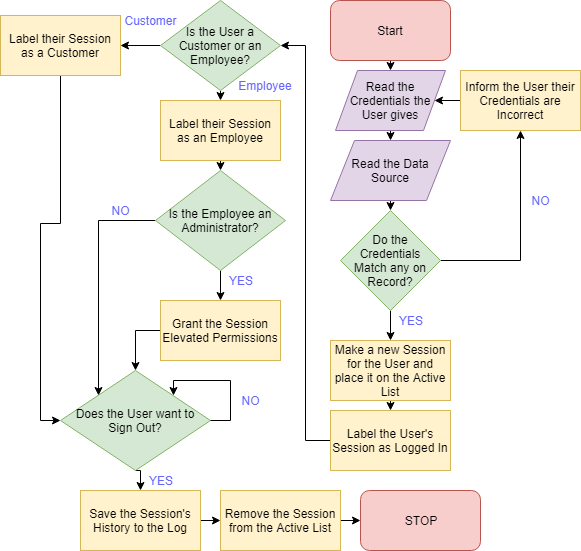
\includegraphics[width=\textwidth]{loginSystem.png}
    \centering
    \end{figure}
    \paragraph{•}
    A Session refers to the user's connection to the host computer; it is persistent while the user remains connected to the web application and can have many properties and pieces of data attached to it.
    The Active List is the conceptual area in memory where the hosting machine will keep track of all the currently active Sessions.
    \newpage
    \paragraph{Store Main Area}
    This page/area represents the forefront of the website as it is presented to the customer, and thus must be "slick" and comprehensive.
    According to my research, I have planned out filtering and sorting features within the page.
    \begin{figure}[h]
    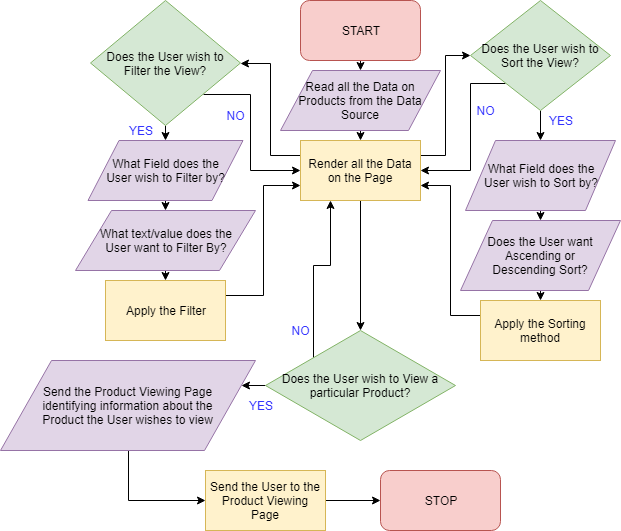
\includegraphics[width=\textwidth]{storefrontMain.png}
    \centering
    \end{figure}
    \paragraph{•}
    The algorithms used for sorting and filtering will be covered in more details in the algorithms section below.
    \newpage
    \paragraph{Product View Page}
    This page will be the "detailed" display of all the information regrading the product.
    It will show a set of images and a written, plain text description.
    Customers will be able to add a given amount of a product to their "cart" there.
    It is \textit{imperative} that the information displayed on this page is plentiful, and very legible.
    \begin{figure}[h]
    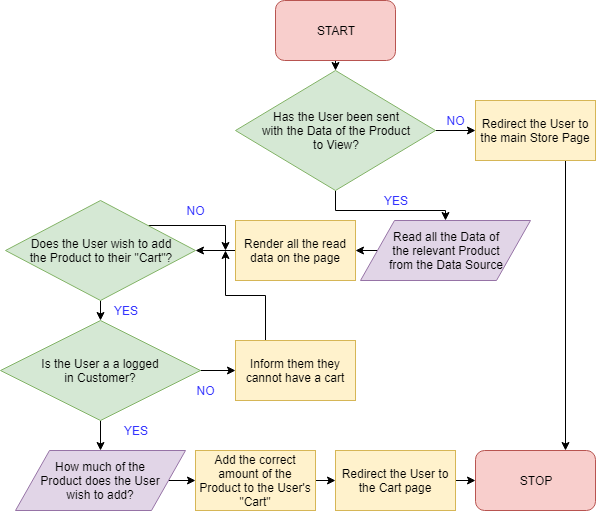
\includegraphics[width=\textwidth]{productPage.png}
    \centering
    \end{figure}
    \paragraph{•}
    The cart should be a collection of products stored in a group labelled with what customer has them in their cart.
    It should be independent of the Sessions so that customers can leave the website or sign out without losing the items in their cart.
    Users who aren't logged in to a customer account may not possess a cart because employees are not authorized to make purchases on the site and people who are not logged in at all may not possess a cart because an account is needed to make a purchase (so purchases are track able).
    \newpage
    \paragraph{Cart Page}
    The cart page shows the customer what they currently have in their cart, lets them edit amounts  and remove products.\\
    More importantly, this is the page where users will make their actual purchases from.
    There are several factors which should be considered in regard to this feature:
    \begin{itemize}
    \item Whether there is enough of all products in the inventory to supply the user's purchase
    \item The user's payment method
    \item The user's delivery address
    \end{itemize}
    After poring over these, I produced the following method.
    \begin{figure}[h]
    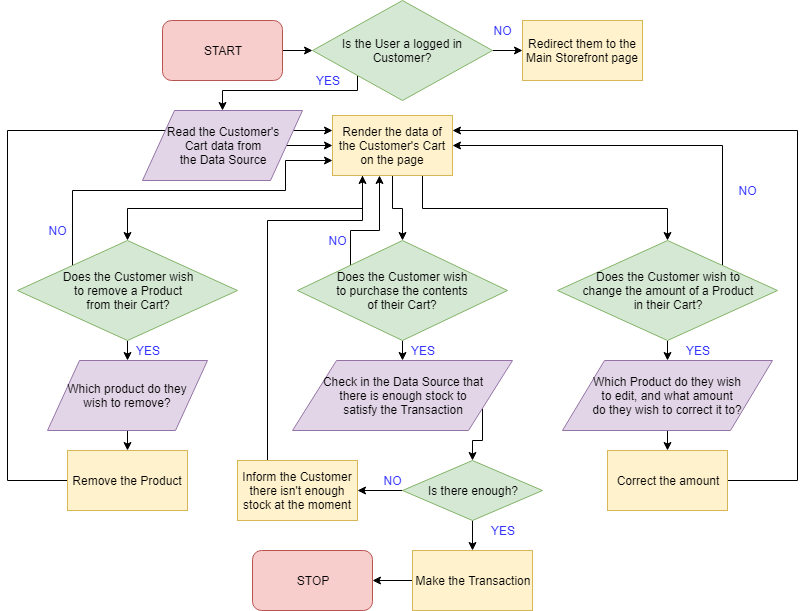
\includegraphics[width=\textwidth]{cartPage.png}
    \centering
    \end{figure}
    \paragraph{•}
    The transaction must be handled individually, as it's own process.
    While I cannot guess yet, managing monetary transactions may well prove to be out of the scope of this project, but this is yet to be proved.
    \newpage
    \paragraph{Physical Market Management Page}
    This page will be where the employee interacts with all features related to managing stock at third party events.
    Tt's appearance could quickly get confusing, so careful UI design is important.
    \begin{figure}[h]
    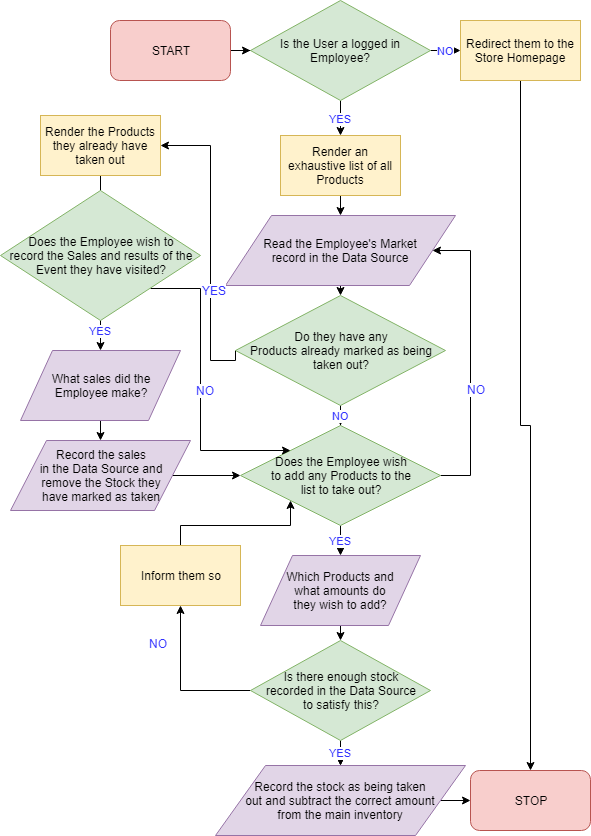
\includegraphics[scale=0.6]{physicalMarket.png}
    \centering
    \end{figure}
    
    \subsection{Algorithms}
    \subsubsection{Quick Sort}
    \paragraph{} One of the complex algorithms I will employ will be a sorting algorithm to sort lists of products to be displayed on the store front in good time.
    I chose the quick sort algorithm for this purpose because it is highly efficient across most datasets, having $O(log(n))$ average complexity and $O(n^2)$ worst case complexity, and because it offers the opportunity to be solved recursively.
    My pseudocode for the algorithm is as follows:
    \begin{lstlisting}[language=psuedocode]

function quicksort(dataset)
    //Contingencies
    switch dataset.length:
        case 1:
            return dataset
        case 2:
            if dataset[1] < dataset[0] then
                dataset[0], dataset[1] = dataset[1], dataset[0]
            endif
            return dataset
    endswitch

    //Find the pivot
    pivotindex = dataset.length / 2
    pivotindex = rounddown(pivotindex)

    //Define the two lists
    list under
    list over

    //Main code block
    for i = 0 to (dataset.length - 1)
        if i == pivotindex then
            continue
        elseif dataset[i] < dataset[pivotindex] then
            under.add(dataset[i])
        elseif dataset[i] >= dataset[pivotindex] then
            over.add(dataset[i])
        endif
    next i

    //Convert to arrays and recur
    array underArray = quicksort(under.toarray())
    array overArray = quicksort(over.toarray())
    
    //Return
    return underArray + dataset[pivotindex] + overArray
endfunction
    \end{lstlisting}
    \paragraph{}
    If the dataset (array) the function is passed is too short, the main code block won't function correctly.
    The first block of code labelled "Contingencies" (beginning line 4) is designed to circumvent this problem; if the function is passed a array of length 1, it will just return it immediately or if it is passed an array of length 2 it will check if they need swapping then return them concatenated into a new array.
    This can also be referred to as the "break case" of the recursive function - it is the place where the function decides whether or not to recur so that the recursion loop isn't infinite.
    \paragraph{}
    The method I chose for finding the pivot in my implementation of quick sort was just to find the element which was halfway through the array; there is much debate over what is the best method, but this one seems the simplest to implement and the most useful for the application at hand.
    I have used rounddown() as a placeholder for a function which rounds down non-integer numbers into integers.
    \footnote{I choose this over rounding up because the arrays are zero based but I expect the lengths to be one based, and this function will compensate for both that and any .5s that may occur in datasets of odd length.}
    \paragraph{}
    When the code refers to the "list" type on lines 18 \& 19, I have called the type list to placehold for the "List" type in C\#, the language I intend to implement this algorithm in.
    A list is an open-ended array which can be appended to and turned into a "true" array at any time.
    \paragraph{}
    Beginning line 23 is the main block of code where the comparisons are made; if the current element is the pivot (checked against the pivot's index as found before) it is skipped, if it is smaller than the pivot it is added to the list of smaller elements and if it is higher or equal then it is added to the list of bigger elements.
    This is the primary logic of quicksort.
    \paragraph{}
    Beginning line 34 is the "recursive case" of the function, i.e. where it recurs (calls itself within itself).
    The function converts the two lists to arrays and passes them to new instances of itself.
    This is powerful because any individual function need only focus on one iteration of the whole sorting process, which makes the code easier to read and understand.
    The algorithm will spawn instances of the function until the break case is tripped, i.e. the array length it is passed is less than 3, when it will just return the array without creating another instance.
    This break case will "travel up" the "stack" of instances and all will return their section of the dataset, sorted, in turn.
    When the initial instance is reached by this phenomenon, it will return the full dataset to the script which called it initially.
    \subsection{Key Variables and Structures}
    Variables are named references to sections of memory.
    They are the label for a data value - referring to them or using them will return you the value of that section of memory.
    Due to this functionality, they are essential to developing a complex program like mine, for storing commonly accessed or changed sections of data and are in fact commonplace in all code scripts for practically all purposes.
    \subsubsection{Global Variables}
    The only variables which need to carry between pages are those related to the system controlling logged in users because all pages need to be able to "tell" information about the user that is viewing them, and all other variables will not be needed by \textit(all) pages.
    These variables will be:
    \begin{itemize}
        \item A string holding the user name of the user that is currently logged in.
        \item A string or boolean representing whether or not the user is an employee or a customer.
        Either of these types could be used; the string would use more memory than necessary but would make the code more understandable whereas the boolean would do the opposite (less memory and less readability).
        \item A boolean holding "true" to show is the user is an administrator, or "false" if they are not.
        Another option to replace both this and the above variable would be something like an Enumerator (a user defined type which can have a set number of enumerable values) which could have the predefined values "Customer", "Employee" and "Administrator" or similar.
        However, using two booleans or a bool and a string makes boolean logic on each page slightly less complicated and reduces the need for iteration where it isn't necessary.
        \item Optionally, a bool showing whether there is a user logged in or the current session is a "guest", ie. not authenticated or formally identified.
        The need for such a variable could be circumvented by simply setting the value of the string holding the user name to be blank or null, but that method could allow people to put exploits in their username string and perform unauthorized and/or unintended acts on the application.
    \end{itemize}
    \subsubsection{Structures}
    The data source is the single key structure in this project.
    It is critical that the data source be able to store all information the website needs, and make it easily accessible and logically organised so that it can be searched, sorted and manipulated.
    To this end, I have chosen to use a relational data base as my data source.
    The additional advantage of using this structure is that within a relational database, the database engine can force referential integrity, which reduces the need for consistency checks at the frontend.
    Within the database I will have six tables, they will be as follows:
    \paragraph{Customers} I have chosen to store customers and employees in separate tables because the data attached to each type is different from the other.
    I am going to investigate the viability of different specific implementations of these tables during development because I do not presently know enough about Microsoft Access to predetermine the method I will use to store customers' data.
    It should, however, contain basic information:
    \begin{description}
        \item[User Name] The user name or handle the customer wishes to be identified by on the site.
        This should be unique.
        \item[Real Name] The real name of the user in some format, so their online account can be easily linked to their real world identity for purposes such as shipping and customer support.
        \item[Password] The private string which the customer uses to verify it is really them whenever they try to log in to the application.
        This information is very sensitive and so I will not store the password verbatim, instead, I will store a hash of the true password (a hash is a value that can be generated from a piece of data, but is generated so that the original data cannot be directly obtained from the hash).
        This means that if the data base's security is breached then attackers will only obtain the hashes, which are useless for logging into the website.
        \item[Address] The address will allow me to implement the feature I described above where the website remembers the customer's delivery infomation for convenience during checkout.
        It could also be used for user verification for customer support.
        \item[Other Personal Info] These could be contact information such as phone numbers or email addresses.
        It is generally helpful to my client's company that this information be attached to their customers, for the aforementioned customer support.
    \end{description}
    \paragraph{Employees}
    The employees table can be a little more concise since not as much personal information is required; that and the inclusion of the administrator boolean are the only differences between it and the customer table.
    \begin{description}
        \item[User Name] The user name or handle the customer wishes to be identified by on the site.
        This should be unique.
        \item[Real Name] This is simply for the sake of simplicity and convenience.
        It could be helpful for identifying employees when a lot are registered.
        \item[Password] This will be a hash of the employee's actual password.
        It will be used for checking their credentials when they try to log in.
        \item[Administrator] This is the boolean variable I described above.
        It will label whether or not the employee is an administrator.
    \end{description}
	\paragraph{Products}
    The products table is very important as it is the table most pages related to the web application's primary function will access.
    \begin{description}
        \item[Product Name] The name of the product; should be unique.
        \item[Type] A string showing whether the product is a clock, coaster or other.
        \item[Stock] An integer storing the amount of the product available in stock (not including the stock which has been taken to a physical market).
        \item[Price] The amount of money, in GBP, that the product will cost a customer.
        Stored as a currency format.
        \item[Creator] The username of the employee who created it.
        This helps with accountability for errors and keeps the history of the database traceable.
        \item[Description] A long string with lots of details about the product which will be displayed on the individual product page.
        \item[Image] Image file(s), one of which will be displayed as the product's thumbnail on the product listing page and all of which will displayed in a "slide show" on the individual product page.
        \item[Band] A string containing the name of the band the product is linked to.
        This allows products to be searched or sorted by what band they are based on.
    \end{description}
    \paragraph{Orders}
    The orders table will record every individual order that has ever been placed on the web application.
    \begin{description}
        \item[ID] This will be an automatically generated number used as the primary key for the database.
        This serves little front-end purpose.
        \item[Date Placed] Quite simply, a string or date format which will store the date and time that the customer placed the order.
        This is essential for statistics, order tracking and customer support.
        \item[Product Ordered] The name of the product which the customer ordered.
        This will be referentially enforced against the names of products registered in the products table.
        \item[Volume Bought] An integer storing how many units of the product the customer ordered.
        \item[Transaction Value] A decimal or price format which stores how much money was requested and received by the application.
        While this could be calculated on the spot whenever the record was accessed, by just multiplying the volume bought by the price in the relevant record in the products table, this method allows for sales or discounted purchases to be stored accurately and eliminates the need to run queries on two different tables to get one piece of data.
        \item[Buyer] The username of the customer who placed the order.
        This should be referntially enforced.
    \end{description}
    \paragraph{Market Items}
    A method to "reserve" items which are taken to a market by an employee is needed; and I have decided to create a separate, simple, table to store those.
    \begin{description}
        \item[Product Name] The name of the product which has been taken out.
        \item[Volume] The amount of the product which has been taken out.
        \item[Employee] The username of the employee who is currently responsible for/in possession of these products.
    \end{description}
    \newpage
    \subsubsection{Intended Implementation}
    \paragraph{Microsoft Access}
    I have chosen the Microsoft Access software to create and manage the database which will support the application.
    Access is freely accessible to me as a student and provides professional level database software which integrates perfectly with my other choices for implementation.
    It allows me to create an automatically enforced relational database which can be queried at any time by any MySQL-compatible code.
    \paragraph{C\#}
    I have chosen the .NET-based language Visual C\# to implement the majority of all logic-based algorithms and scripts in this project.
    My reasoning for this is:
    \begin{itemize}
        \item I am already familiar with C\# and it's syntax, types and object-oriented problem solving method.
        This reduces the possibility of coming across problems I haven't encountered before meaning development wil hopefully be faster.
        It is still inevitable that I will encounter such obstacles, but C\# should throw fewer than other choices.
        \item The .NET foundation provides the excellent ASP.NET libray which contains a set of elements for .NET languages to be used for web development.
        ASP.NET comprises a set of JavaScript elements that imitate HTML elements while simultaneously giving them "hooks" (methods and properties) which are accessible by the .NET-based language behind each page.
        \item ASP also provides the functionality of Master pages, which are a perfect method of implementing the base layouts I describe in a later section.
        These are pages with set elements on them which all pages inherit from, and add their own content to.
        \item C\# integrates well with the Microsoft Access database engine with the use fothe Microsoft-provided OleDB library, which contains many functions for running powerful SQL queries on MS access databases.
    \end{itemize}
        \subsection{Usability Features}
    \paragraph{}
    Since this project is a web application with a public-facing GUI, usability features are a vital consideration at all stages of development.
    The primary focus of that consideration will be UI layout and design; all pages must only show what they need to, with no excess information, in a clear and concise format.
    \paragraph{Base Layout}
    To this end, I intend to have a "base layout" for all pages.
    This will be a blank layout with minimal features (only those which all pages will require) and a large amount of blank space for the content of each page to be placed in.
    There will be two iteration of this "base layout" - one for all employee-only pages, and one for all others.
    The two will have starkly colour schemes so they are clearly distinguished when viewing them in order to clearly show when an employee is viewing a customer area or an exclusive employee only page.
    \paragraph{Nav-Bar}
    A nav bar is an area at the top of the page containing links for navigating the web application.
    These links will be relevant on all pages, they will include a link to the home page, login page and product browsing page; or the statistics page and market page on the employee pages.
    It will also show an element showing the real name of the currently logged in user, with options to sign out and view their profile.
    If no user is logged in, it will show a login button in place of this.
    I plan to implement this feature as the central component of both base layouts.
    \paragraph{Content}
    This is a reserved area of the page where the unique content of each page will be shown, according to the page the user is viewing, for example: on the analytics page graphs will be shown whereas on the product browsing page the product list will be shown.
    It will be the only place each individual page is allowed to place elements and content.
    \paragraph{Background}
    While this may not strictly be a usability "feature", I think there should be an image background at the edges of the page to break up the monotonous colours.
    This has the dual advantage of both making the website more pleasing to look at and easier to read.
    \paragraph{}
    Since this is a web application, the best method to implement these features is, without a doubt, Cascading Style Sheets.
    CSS is a styling language that dictates the appearance, colour and layout of web pages.
    I have chosen it because:
    \begin{itemize}
        \item It allows powerful control of many aspects of web pages as mentioned above with only a few lines of code
        \item It is simple to read, learn and understand because it has little to no syntax variation
        \item It can set presets for elements of particular user defined classes, allowing it to retain consistency across the site with minimal extra effort
    \end{itemize}
    \newpage
    \subsubsection{Customer Base Layout}
    \begin{figure}[h]
        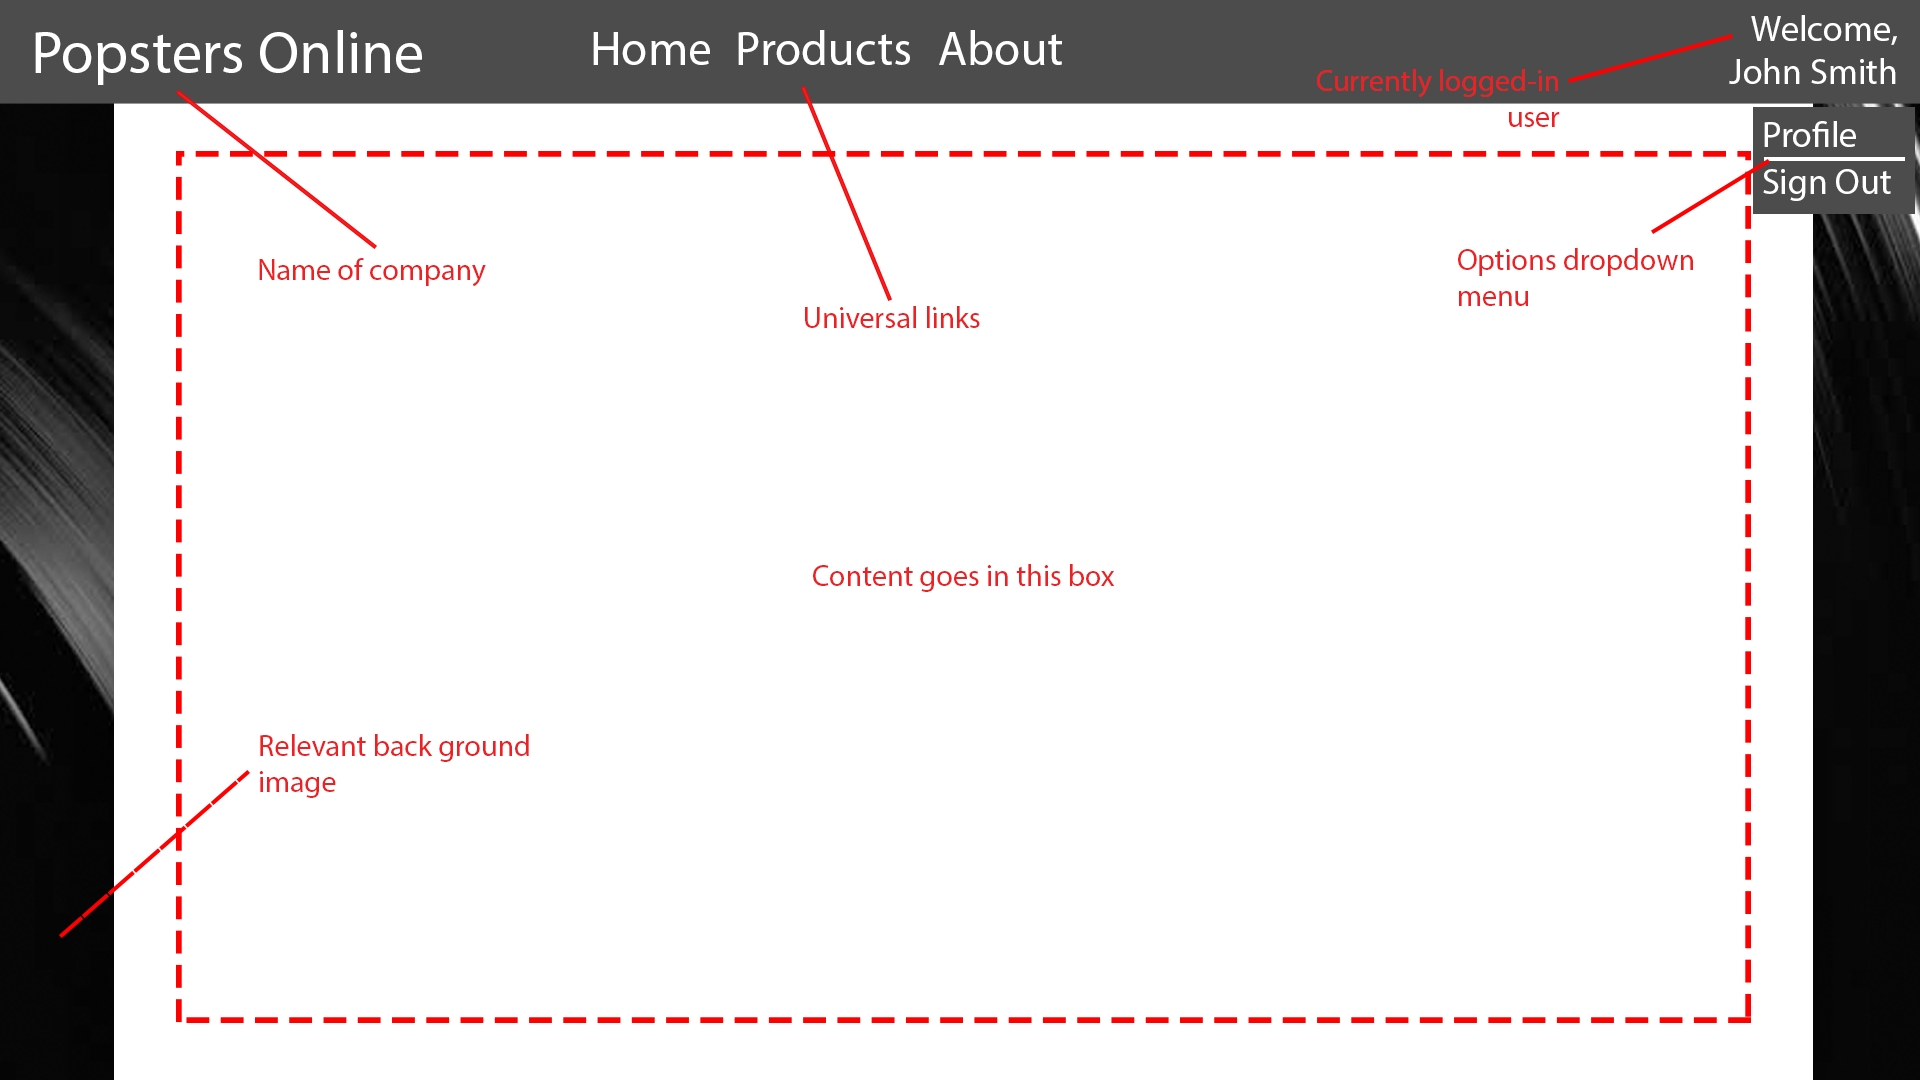
\includegraphics[width=\textwidth]{customerBasic.png}
        \centering
    \end{figure}
    \paragraph{}

    \newpage
    \subsubsection{Employee Base Layout}
    \begin{figure}[h]
        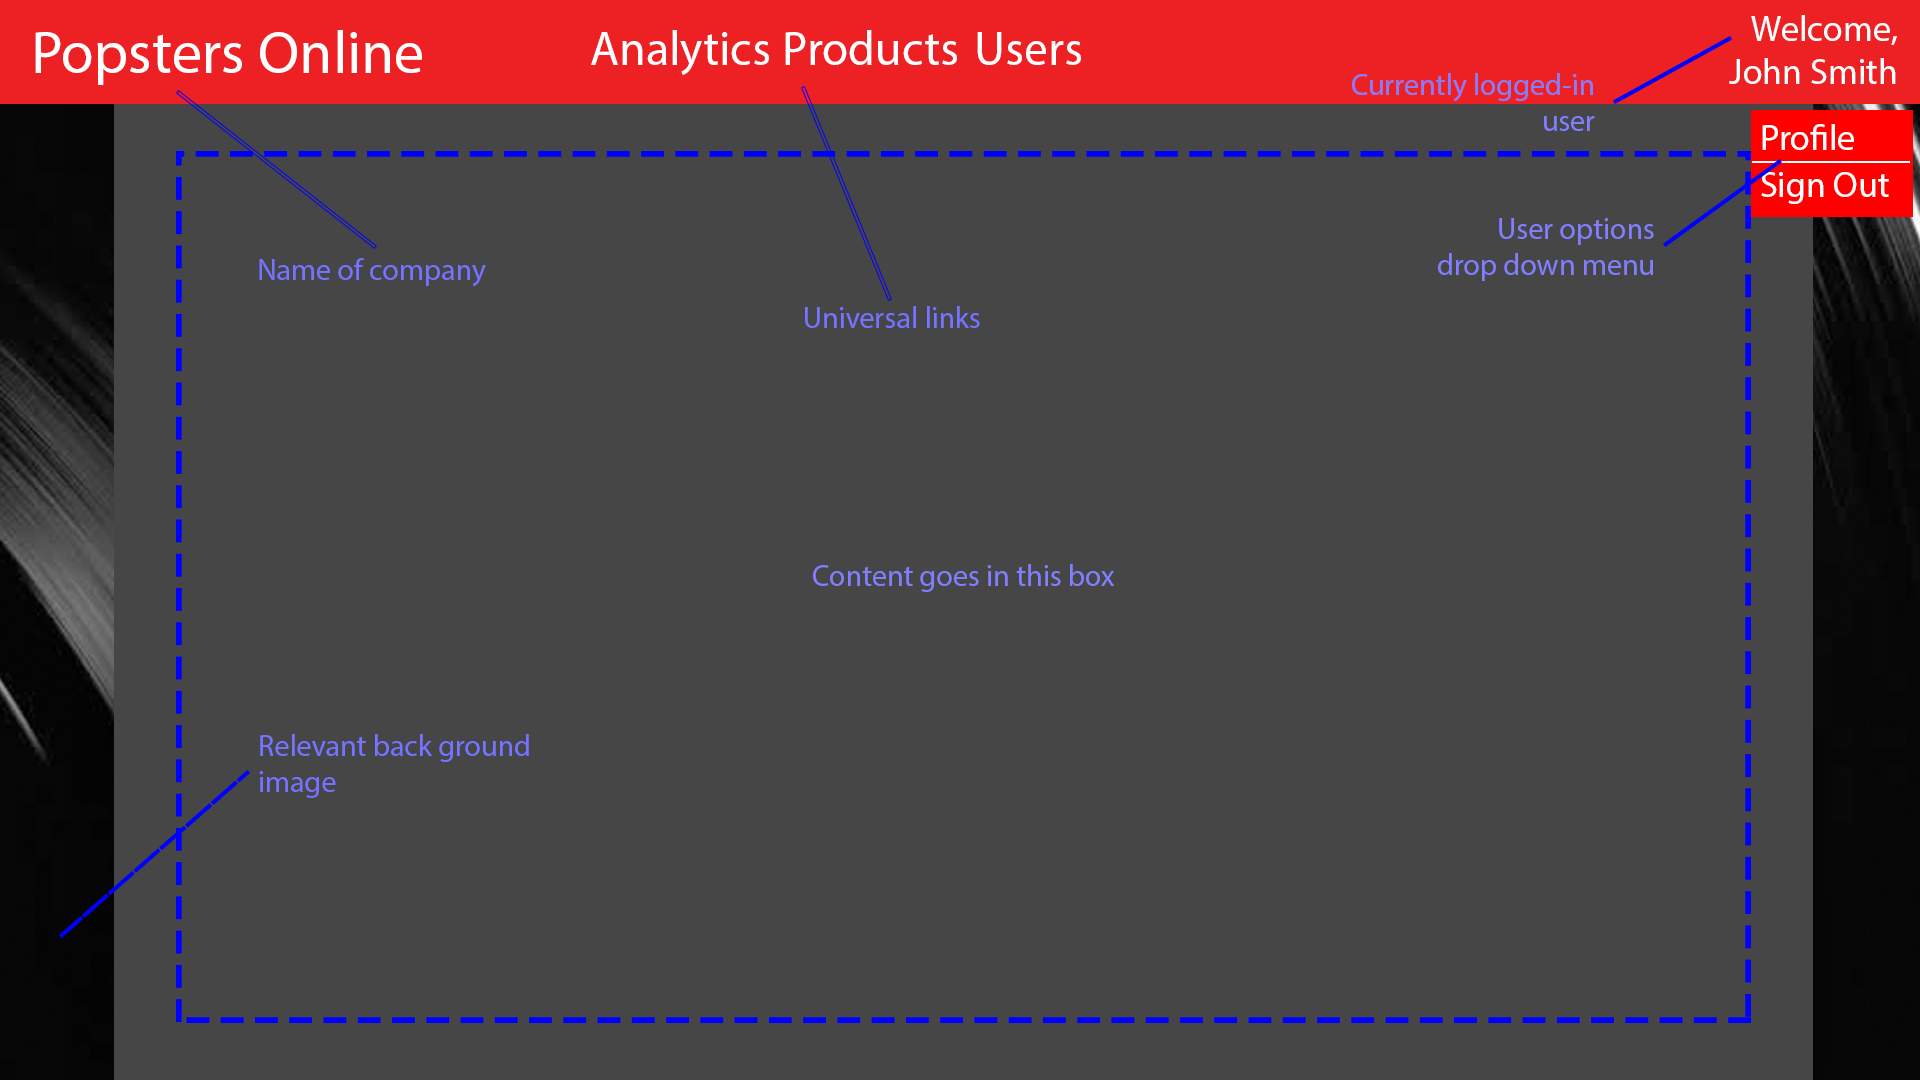
\includegraphics[width=\textwidth]{employeeBasic.png}
        \centering
    \end{figure}
    \paragraph{}

    \subsection{Test Data}
    
    
    \section{Iterative Development}
    \subsection{Data Base}
    Above, I described the contents of each table in the database.
    This section is here to provide a visualisation of the relationships between the tables with a screenshot of the Access relationships screen:
    \begin{figure}
        \centering
        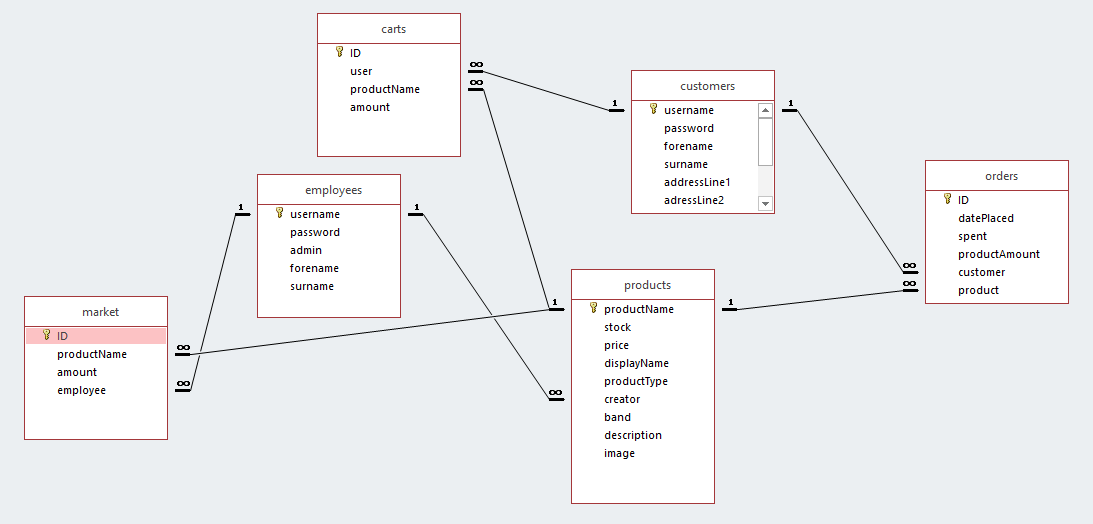
\includegraphics[width=\textwidth]{dataBaseScreen.png}
    \end{figure}
    \subsection{Annotated Code (Initial Solution)}
    \subsubsection{Preface}
    \paragraph{Code Structure}
    My project is a web application, with the web pages written in ASP.NET and the logic behind them in Visual C\#; as such, an optimal structure and organisation of the code is available.
    Points to remember:
    \begin{enumerate}
        \item All pages are composed of a .aspx file, and a .cs file.
        The .aspx file stores the markup language style code (ASP) that dictates what elements are permanently present on the page, and all their properties.
        The .cs file stores the logic attached to those elements and contains all the C\# code which can refer to all elements present on the ASP page as if they were ordinary objects; it always contains a predefined method called Page\_Load which will be called when the page loads.
        \item There is a master file (in my case two) which all pages inherit from.
        This has common elements like the nav-bar and the content at the bottom of the page.
        It, just like all other pages, has a .cs file attached containing code which applies elements on that page, which are active on all pages dependant on that master file.        
    \end{enumerate}
    \paragraph{Sessions}
    Within ASP, the Session object refers to a class containing an array of objects which are universal across all pages - a set of global variables, if you will.
    This is helpful for implementing code which keeps the user authenticated, as described in the design section and is conveniently named the same thing.
    There are four variables stored in it which I refer to constantly:
    \begin{description}
        \item[isLoggedIn] This is a boolean simply representing whether there is currently a user logged in.
        \item[currentUser] This is a string storing the username of the user currently logged in.
        It's default value (i.e. when no one is logged in) is "" (nothing).
        \item[userType] This is another string storing whether the logged in user is an employee, or a customer.
        It's default value is also "".
        \item[userIsAdmin] A boolean storing whether the logged in user is an administrator.
        Default value false.
    \end{description}
    \newpage
    These are all the classes which contain code needed by many different pages for similar reasons.
    They are not in the master files because not all pages need them, and those that do will likely not need all of them.
    Instead, they are grouped into their own .cs file in order to keep them accessible and grouped together without any other logic making them more difficult to read and change.
    \newpage
    \subsubsection{Logging}
    The following code controls all the logging of all actions in the software, all log entries are processed through this class.
    This is not a webpage, this is just a section of shared code.
    \begin{lstlisting}[language=C]
public class customLogging
{
    public static void newSession()
    {
        string result;
        string dividerASCII = "------------------------------------------";
        result = dividerASCII + generateTimestamp() + dividerASCII;
        writeEntry("");
        writeEntry(result);
    }

    public static void newEntry(string entryText)
    {
        string result = generateTimestamp() + " " + entryText;
        writeEntry(result);
    }

    public static void newException(Exception except)
    {
        string result = generateTimestamp() + " An error occurred in " + except.Source + " with message " + except.Message;
        writeEntry(result);
    }

    private static void writeEntry(string entryText)
    {
        try
        {
            using (StreamWriter logFile = new StreamWriter(@"\\albert \2011\R04637\Computer Science\coursework\mainCoursework\App_Data\log.txt", true))
            {
                logFile.WriteLine(entryText);
            }
        }
        catch (IOException)
        {
            using (StreamWriter logFile = new StreamWriter(@"C:\Users\Edward\Source\Repos\coursework\mainCoursework\App_Data\log.txt", true))
            {
                logFile.WriteLine(entryText);
            }
        }
    }

    private static string generateTimestamp()
    {
        string output = "[" + Convert.ToString(DateTime.Now) + "]";
        return output;
    }
}
    \end{lstlisting}
    The methods are as follows:
    \paragraph{writeEntry} The method that writes the text passed to it to the log file.
    Here, I have used a try-catch statement to bypass a problem I encountered when working on this project between two workstation in different locations - at school and at home.
    Since the application does not run out of the directory containing the pages it is showing (the same directory which contains the logfile) because it executes on the pre installed IIS express server, referential file paths serve no purpose.
    My solution to this was to simply try the file path which would ordinarily contain the logfile on the school hard drive, and switch to that at home if it failed.
    \\
    The method takes a string containing the text it should enter into the file, opens a StreamWriter class (the system class for writing to binary files) and uses it to send the requested text to the file.
    \paragraph{generateTimestamp} This is a string method that returns the current time with square brackets around it, ready to be prefixed onto a log entry.
    \paragraph{newSession} A void method which puts a dividing line in the log file indicating that the server has just started, and the history below it until the next divider is a new instance of the server.
    It also tags it with generateTimestamp's output to mark when the session started.
    This method is only called by the master page constructor.
    \paragraph{newEntry} Another void method which creates a string from the string it is passed and the output of generateTimestamp, and writes it to the log with writeEntry.
    \paragraph{newException} Similar to newEntry but it writes an exception's contents to the log.
    It uses the properties of the exception passed to it "source" and "message" to generate an appropriate entry to the log, timestamp it and write it.
    \newpage
    \subsubsection{Custom Security}
    The customSecurity class only covers MD5 hashing and SQL injection checking.
    \begin{lstlisting}[language=C]
public class customSecurity
{
    public const string sanitizeErrorMessage = "All fields must be full. The (, ), +, -, = and ' characters are not allowed in ANY fields";

    public static bool sanitizeCheck(string[] input)
    {
        bool isClean = true;
        foreach (string i in input)
        {
            if (i.Contains("(") || i.Contains(")") || i.Contains("'") || i.Contains("=") || i.Contains("-") || i.Contains("+"))
            {
                isClean = false;
                break;
            }
            if (i == "")
            {
                isClean = false;
                break;
            }

        }
        return isClean;
    }

    public static string generateMD5(string input)
    {
        var md5 = System.Security.Cryptography.MD5.Create();
        byte[] inputBytes = System.Text.Encoding.ASCII.GetBytes(input);
        byte[] hash = md5.ComputeHash(inputBytes);
        string output = "";
        for (int i = 0; i < hash.Length; i++)
        {
            output = output + hash[i].ToString("x2");
        }
        return output;
    }
}
    \end{lstlisting}
    \paragraph{sanitizeErrorMessage}
    A custom error message stored so that error returns can use it.
    This exists to retain consistency, i.e. all returns show the same message when SQL - relevant characters are found.
    \paragraph{sanitizeCheck}
    According to my success criteria, the application must adequately protect the users' data.
    A common method of trying to breach application which use SQL to interact with their databases is called "SQL Injection" - this is when an attacker enters an SQL command into an input they think will be checked against the database.
    This can be used to issue commands to the database without correct authentication - attackers can log in, drop tables and commit other destructive actions.
    The most common way to prevent this is referred to as Sanitization, when inputs are checked for characters that could be used in an SQL statement and either remove them or refuse the input if they are found.
    I have adopted this as no inputs require any of these characters as part of their function; this code takes an array of input box contents and returns true or false depending on if any of those inputs contain SQL sensitive characters (specifically (,),=,-,+).
    It also serves to make inputs required as it will return false if any of them are blank.
    \paragraph{generateMD5}
    As stated in the key structures section of my design, all passwords stored in the database will be hashed so in the event that they are comnpromised, the password values are of little use.
    \\
    The code uses the System.Security.Crypography library to access the algorithms required to generate MD5 hashes from byte data.
    The function takes a string and creates a new instance of the MD5 class from the cryptography library.
    It converts the input into an array of bytes using the System.Text.Encoding.ASCII class (which changes ASCII values into byte data, i.e. strings into binary)
    Another array of bytes is generated using the ComputeHash method of our Cryptography.MD5 instance (called md5).
    The string output is defined and assigned as "" (this is because the next for loop requires an already existing string to append to).
    A for loop is run up to the length of the array of bytes (the output data) which appends the string output with each byte using the .ToString method which most objects in C\# possess.
    The "x2" argument specifies that each string output should be capitalised (I use this for consistency).
    \newpage
    \subsubsection{Data Set}
    \paragraph{}
    C\# and the .NET framework in general provide DataSets for the use of developers to easily interface with a data source.
    The DataSet automatically generates code using OleDB (the Microsoft database engine) for each query you add to it.
    I have constructed one central DataSet which holds all my tables and several queries for each.
    The SQL query statements will be shown and annotated as they are used.
    The full dataset is shown below:
    \begin{figure}[h]
        \centering
        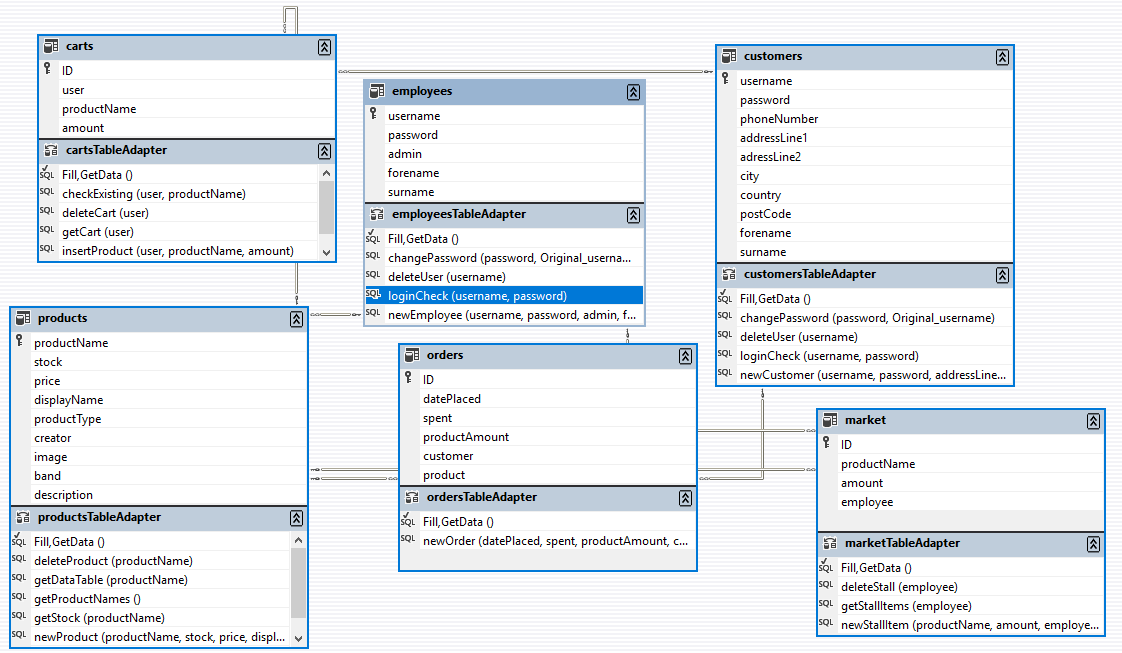
\includegraphics[width=\textwidth]{defaultDataSet.png}
    \end{figure}
    Each table is shown in a box, with the adaptor (the containing object with all the user-defined queries in it) in an adjoining box below that
    Data relationships are shown with lines connecting the tables, data fields by rows in the table box and queries in the adaptor box.
    \newpage
    \subsubsection{Log In}
    \begin{lstlisting}[language=C]

public partial class customerLogin : System.Web.UI.Page
{
    protected void Page_Load(object sender, EventArgs e)
    {
        if (Convert.ToString(Session["isLoggedIn"]) == "True")
        {
            Server.Transfer("~/default.aspx", false);
        }
    }

    protected void submitCustomerCredentialsButton_Click(object sender, EventArgs e)
    {
        if (customSecurity.sanitizeCheck(new string[] { customerUsernameBox.Text, customerPasswordBox.Text }))
        {
            string attemptedName = customerUsernameBox.Text;
            using (var checkCredentials = new defaultDataSetTableAdapters.customersTableAdapter())
            {
                if (checkCredentials.loginCheck(attemptedName, customSecurity.generateMD5(customerPasswordBox.Text)) != null)
                {
                    Session["isLoggedIn"] = "True";
                    Session["currentUser"] = attemptedName;
                    Session["userType"] = "customer";
                    Session["userIsAdmin"] = "False";
                    customLogging.newEntry("Customer " + attemptedName + " logged in");
                    Server.Transfer("~/default.aspx", false);
                }
                else
                {
                    customerLoginReturnLabel.Text = "The Username or Password is incorrect.";
                    customLogging.newEntry("Someone attempted to login as a customer with username '" + attemptedName + "' but the credentials were incorrect");
                }
            }
        }
        else
        {
            customerLoginReturnLabel.Text = customSecurity.sanitizeErrorMessage;
        }
    }

    protected void registerButton_Click(object sender, EventArgs e)
    {
        Server.Transfer("registerCustomer.aspx", false);
    }

    protected void employeeRedirect_Click(object sender, EventArgs e)
    {
        Server.Transfer("employeeLogin.aspx", false);
    }
}
    \end{lstlisting}
    \paragraph{}There are two log in pages in my project, one for the customers and one for the employees; because the customer and employee tables are seperate, it is more convenient to seperate the logic for each table into two seperate pages/files.
    In terms of appearance, the two pages are identical but for the inclusion of a button on the customer page which redirects the user to the customer register page.
    Otherwise, both pages contain a text box for the user name of the user and their password (customerUsernameBox and customerPasswordBox or equivalent), a submit credentials button (submitCustomerCredentialsButton or equivalent) and finally a button to redirect the user to the employee login or customer login as appropriate (employeeRedirect or equivalent).
    \paragraph{Page\_Load} This page should not be accessible by people that are already logged in, as logging in again is unnecessary if they are already logged in and could cause unforeseen problems.
    This checks the session "isLoggedIn", and if it tagged as true then it redirects the user to the relevant homepage with the Server.Transfer method (this is used on almost all pages to redirect people - it's arguments are the path of the page to redirect to and whether to "preserve" the form it is currently loading, for my purposes this is always false).
    In the employee file, it will redirect to the employee homepage, which will then redirect to the customer homepage if it is a customer logged in.
    \paragraph{submitCustomerCredentialsButton\_click} A method called when the submit button is clicked (ASP automatically generates blank methods linked to each button's onclick event, comprised of the name of the button followed by "\_click").
    Within this method, I have used two nested if statements with boolean logic to check the inputs for validity.
    The first ensures that both input boxes are free of SQL characters with customSecurity.sanitizeCheck and returns the appropriate error message to the return box if not, while the second runs a query against the database:
    \begin{lstlisting}[language=SQL]

        SELECT COUNT(*) AS Expr1
        FROM customers
        GROUP BY username, [password]
        HAVING (username = ?) AND ([password] = ?)
    \end{lstlisting}
    This query will return a DataRow type if an entry with matching credentials is found, and null if not.
    The boolean logic in the if statement checks if something was returned, and if it was it runs the code within it.
    If null is returned then it will not run anything and change the error message label to inform the user they have input incorrect credentials.
    The code within the if statement sets all the appropriate session data as described previously, using the username string the user gave as the username and setting the administrator \& type values to false and customer respectively on this page.
    It will also log the user entering the site.
    On the employee page, lines 24 to 26 are replaced with:
    \begin{lstlisting}[language=C]

        Session["userIsAdmin"] = Convert.ToBoolean(loginCheck);
        if (Convert.ToBoolean(Session["userIsAdmin"]))
        {
            customLogging.newEntry("Admin " + attemptedName + " logged in");
        }
        else
        {
            customLogging.newEntry("Employee " + attemptedName + " logged in");
        }
        Server.Transfer("~/staffOverview.aspx", false);
    \end{lstlisting}
    The changes this code introduces are that the return of the query is converted into a boolean with the default static class Convert - this works because the query run for that page is
    \begin{lstlisting}[language=SQL]

        SELECT admin
        FROM employees
        GROUP BY username, [password], admin
        HAVING (username = ?) AND ([password] = ?)
    \end{lstlisting}
    Which returns just the value of the admin field instead of the whole DataRow so the only value for Convert to operate on is the one we want.
    The resulting value is stored in the userIsAdmin session.
    The same session is immediately checked again to decide what to post to the log; if it returns true then the log is told an administrator logged on and if false that an employee logged on.
    The last line redirects the newly-logged in user to the staff overview page instead of the customer home page.
    \newpage
    \subsubsection{Product Class}
    My project needs to deal with lots of information about the products of the client constantly as part of it's base function.
    The code which deals with this is best abstracted enough to be omni-purpose across the site, with little modification needed to use it on different pages for different purposes.
    Most pages related to products need to be able to display a list of products which can be sorted and filtered - to this end I decided to write a instantiable class representing one product and attach code to it that would let it gather it's data for itself.
    Eventually, I wrote the following:
    \begin{lstlisting}[language=C]
public class product
{
    private defaultDataSetTableAdapters.productsTableAdapter adapter = new defaultDataSetTableAdapters.productsTableAdapter();

    private productStruct ProductInfo = new productStruct();
    public productStruct productInfo
    {
        get
        {
            return ProductInfo;
        }
    }
    public int newStock { get; set; }

    public product(string iniName)
    {
        getData(iniName);
    }
    public product(DataRow row)
    {
        ProductInfo.productName = Convert.ToString(row[0]);
        ProductInfo.displayName = Convert.ToString(row[3]);
        ProductInfo.stock = Convert.ToInt32(row[1]);
        ProductInfo.price = Convert.ToDecimal(row[2]);
        ProductInfo.band = Convert.ToString(row[7]);
        ProductInfo.description = Convert.ToString(row[8]);
        ProductInfo.imagePath = Convert.ToString(row[6]);
        ProductInfo.type = Convert.ToString(row[4]);
    }
    
    public void saveStock()
    {
        adapter.updateStock(newStock, ProductInfo.productName);
        ProductInfo.stock = newStock;
        newStock = 0;
    }

    public void refresh()
    {
        getData(ProductInfo.productName);
    }

    private void getData(string searchName)
    {
        var rows = adapter.getDataTable(searchName);
        DataRow row = rows[0];
        ProductInfo.productName = searchName;
        ProductInfo.displayName = Convert.ToString(row[3]);
        ProductInfo.stock = Convert.ToInt32(row[1]);
        ProductInfo.price = Convert.ToDecimal(row[2]);
        ProductInfo.band = Convert.ToString(row[7]);
        ProductInfo.description = Convert.ToString(row[8]);
        ProductInfo.imagePath = Convert.ToString(row[6]);
        ProductInfo.type = Convert.ToString(row[4]);
    }
}
    \end{lstlisting}
    \paragraph{Properties and Variables}
    A property in C\# is an attribute of a class which allows outside code to read and write to objects within it.
    This can be used to make certain values read-only or write-only, or attach code to such events to control what conditions the object(s) can be accessed under.
    It is good practice to implement properties instead of tagging objects within as public because it ensures outside code cannot accidently or deliberately interfere with the objects within the class; while I will be the only contributor to this application's codebase this is not strictly necessary because I know how the class works and don't need to interfere with it, it remains good practice to implement.
    The properties and variables defined in lines 3 to 13 are as follows:
    \begin{itemize}
        \item \textbf{adapter} is the adaptor which the product will use to pull information from.
        \item \textbf{ProductInfo} a custom structure which holds all the information about the product in an uncomplicated, grouped object.
        It's structure is:
        \begin{lstlisting}[language=C]
    public struct productStruct
    {
        public string productName;
        public string displayName;
        public int stock;
        public decimal price;
        public string band;
        public string description;
        public string imagePath;
        public string type;
    }
        \end{lstlisting}
        \begin{itemize}
            \item productName is the camel case name of the product - camel case does not contain spaces and capitalizes the first letter of all words/components but the first.
            I chose this because it maximizes compatibility since it doesn't have any spaces, which can make string manipulation on it easier, and so that strange capitalizations won't allow duplicate products in the data base.
            Also, it is in keeping with my method of using camel case for all my variables and objects in my code.
            \item displayName is the original name the employee who created the product set as the name.
            \item stock is an integer value showing how much stock is left in the inventory.
            \item price is a decimal detailing how much, in GBP, one unit of the product costs.
            \item description is a written description of the product which is defined when the product is created.
            \item imagePath is a file path to the image of the product.
            It should ideally be images/productname.png.
            \item type is the type of product it is, i.e. coaster or clock.
        \end{itemize}
        An additional advantage is that using a struct like this allows me to assign a name to each field instead of having to check by index.
        \\
        \item \textbf{productInfo} is the property used to access the information in ProductInfo.
        It is read only.
        \item \textbf{newStock} This is a simple integer that can be read or written to which a later method will use to change the stock value of a product in the database.
    \end{itemize}
    \paragraph{Constructors}
    In C\#, constructors are declared with "public objectName(arguments)", without a type specifier and with the same name as the parent object.
    There are two contructors in this class - they are overloaded (i.e. the compiler chooses which one to use based on what parameters are given when the object is instantiated):
    \begin{enumerate}
        \item Beginning line 15, the base constructor takes a string holding the productName of the product to load into the new instance.
        It runs the getData() method using this, explained below.
        \item Beginning line 19, the secondary constructor takes a full datarow which would typically be returned by a DataSet query and assigns all of the information in productStruct to the correct fields in that row.
    \end{enumerate}
    \paragraph{Methods}
    There are three methods in the product class:
    \begin{itemize}
        \item \textbf{saveStock} uses adaptor to write the value of newStock to the database with the query updateStock, which consists of:
        \begin{lstlisting}[language=SQL]
    UPDATE products
    SET stock = ?
    WHERE (productName = ?)
        \end{lstlisting}
        This changes the value of the stock field in all entries where productName matches what is given.
        saveStock also updates the stock value in ProductInfo and resets the value of newStock to 0.
        \item \textbf{refresh} runs getData again using the productName variable in ProductInfo.
        \item \textbf{getData} is a private method for use only within the class which runs the query getDataTable using adaptor.
        getDataTable contains:
        \begin{lstlisting}[language=SQL]
    SELECT productName, stock, price, displayName, productType, creator, [image], [band], description
    FROM products
    WHERE (productName = ?)
        \end{lstlisting}
        This searches for productName in the table and returns the entire contents of the table when it finds a match.
        getData uses that information to populate ProductInfo using the appropriate data fields.
    \end{itemize}
    The product class itself is relatively barebones since most of the logic related to organising and presenting products is contained in later objects.
    \newpage
    \subsubsection{productPanel Class}
    I needed a way to show products consistently across all pages and manually writing the code for displaying products on every page that needed it would take more time and be less efficient than alternative solutions.
    To accomplish this, I wrote a class which inherits from the ASP.NET Panel, giving me the advantage of just being able to add the object as it is to forms so it will just render itself.
    \begin{lstlisting}[language=C]
public class productPanel : System.Web.UI.WebControls.Panel
{
    public productStruct info;
    public productPanel(productStruct productInfo)
    {
        info = productInfo;

        this.CssClass = "productDisplayPanel";
        this.ID = info.productName + "Panel";

        Image displayedImage = new Image()
        {
            CssClass = "productImage",
            ID = info.productName + "ImageTag",
            ImageUrl = info.imagePath,
            Height = 400,
            Width = 400
        };
        displayedImage.Attributes.Add("runat", "server");
        this.Controls.Add(displayedImage);
        this.Controls.Add(new LiteralControl("<br />"));

        Label nameTag = new Label()
        {
            CssClass = "nameTag",
            Text = info.displayName,
            ID = info.productName + "NameTag"
        };
        nameTag.Attributes.Add("runat", "server");
        this.Controls.Add(nameTag);
        this.Controls.Add(new LiteralControl("<br />"));

        Label priceTag = new Label()
        {
            CssClass = "priceTag",
            Text = "£" + commonClasses.common.formatPrice(info.price),
            ID = info.productName + "PriceTag"
        };
        priceTag.Attributes.Add("runat", "server");
        this.Controls.Add(priceTag);

        Label stockTag = new Label()
        {
            CssClass = "stockTag",
            ID = info.productName + "StockTag"
        };
        if (info.stock == 0)
        {
            stockTag.Text = "Out of stock";
        }
        else
        {
            stockTag.Text = Convert.ToString(info.stock) + " in stock";
        }
        stockTag.Attributes.Add("runat", "server");
        this.Controls.Add(stockTag);
        this.Controls.Add(new LiteralControl("<br />"));

        Label descriptionTag = new Label()
        {
            CssClass = "descriptionTag",
            Text = Convert.ToString(info.description),
            ID = info.productName + "DescriptionTag"
        };
        descriptionTag.Attributes.Add("runat", "server");
        this.Controls.Add(descriptionTag);
        this.Controls.Add(new LiteralControl("<br />"));
    }
}
    \end{lstlisting}

    \paragraph{Properties}
    The only property in this class is productInfo, which is just a productStruct initialized in the constructor.
    \paragraph{Contructor}
    This class has only one constructor, which serves a double purpose as the only method in the class.
    The constructor initializes a set of controls which together make up the whole panel and contain all information the panel should display.
    First, the ID and CssClass of the panel itself using the dynamic referrer "this".
    For each individual control:
    \begin{enumerate}
        \item The ID and CssClass are set.
        The ID is set to be the name of the product the panel is being generated ofr appended with the name of the control (for the panel, an example ID would be "sampleClock3Panel").
        The CSS class is simply the name of the object because all similar objects need the same CSS class to have the same styling applied to them.
        \item Specific properties for each control are set - see below for these.
        \item The control has the runat Attribute set to "server" using Attributes.Add() so that it runs server-side, not client-side, which would cause persistency problems.
        \item The control is added to the panel's controls array using this.Controls.Add() - the controls array is an array in productPanel inherited from Panel which contains all the controls which are displayed within the panel.
        \item An HTML $<$br /$>$ (breakline, essentially a manual "return" key) is added by instantiating a LiteralControl in order to create some space between elements.
    \end{enumerate}
    \paragraph{}
    The individual controls are:
    \begin{itemize}
        \item \textbf{displayedImage} is the thumbnail (small cover image) for the product.
        It is set to display the image at the path at the imagePath property of the info productStruct and to be 500\*500 so all thumbnails are the same size.4
        \item \textbf{nameTag} is the label which will show the name of the product.
        It's Text property is set to the displayName property of info.
        \item \textbf{priceTag} displays the price of 1 unit of that product.
        It's Text property is set to the stored price of the product from info and prefixed with a "£" character.
        \item \textbf{stockTag} is a label which just shows the integer value of how much of that product is left in the inventory.
        It's Text property is set to the stock value of info.
        \item \textbf{descriptionTag} is a label which will hold the description of the product.
        It's Text property is set to the description of the product using info.
    \end{itemize}
    \newpage
    \subsubsection{productList Class}
    This class contains all the logic for sorting, filtering and otherwise comparing products.
    Since the class is extremely large, I have split it up into groups of similar functions; each section has an accompanying code block, all of which are in order.
    I have omitted the class declaration to make the beginning and end sections easier to read, all of the following is encapsulated in ordinary "class productList {}" tags.
    \paragraph{Properties and Variables}
    \begin{lstlisting}[language=C]
		private defaultDataSetTableAdapters.productsTableAdapter adapter = new defaultDataSetTableAdapters.productsTableAdapter();
		private product[] masterList;
		private product[] WorkingList;
		public product[] list
		{
			get
			{
				return WorkingList;
			}
		}
    \end{lstlisting}
    \begin{itemize}
        \item \textbf{adapter} is, as before, the adapter the productList will use to interface with the database.
        \item \textbf{masterList} is one of two arrays of type product; this one stores the whole contents of the database table when the class is initialized.
        The class won't change the contents of this once it is initialized or it is specifically instructed to.
        \item \textbf{workingList} is the "primary" product array; it is copied from the master list upon initialization then all filtering and sorting is applied to it.
        The advantage of this method is that when the sort or filter needs to be reset, the database does not have to accessed twice which would make the application slower.
        \item \textbf{list} is the property allowing outside access to the working list.
        The master list is private with no property to prevent outside code from interfering with the contents of it because if it did, productList might not function correctly.
    \end{itemize}
    \paragraph{Basic Methods and Constructors}
    The class has a large amount of constructor overloads to account for all possible situations which serve to make it more adaptible.
    It can initialize using an array of products, an array of the names of products, a DataTable of products and, by default, from all the products in the table.
    Many of these features may prove to be redundant later and I may not use some so it is unlikely all these construction methods will survive into the finished project.
    \begin{lstlisting}[language=C]
public void resetWorkingList()
{
    WorkingList = masterList;
}

public Panel[] generateControls()
{
    Panel[] result = new Panel[WorkingList.Length];
    for (int i = 0; i < WorkingList.Length; i++)
    {
        result[i] = new productPanel(WorkingList[i].productInfo);
    }
    return result;
}

public void setWorkingList(product[] array)
{
    WorkingList = array;
}

public productList()
{
    var data = adapter.GetData();
    int i = 0;
    masterList = new product[data.Rows.Count];
    foreach (DataRow row in data.Rows)
    {
        masterList[i] = new product(row);
        i++;
    }
    WorkingList = masterList;
}
public productList(string[] productNames)
{
    int i = 0;
    foreach (string str in productNames)
    {
        masterList[i] = new product(str);
        i++;
    }
}
public productList(DataTable data)
{
    int i = 0;
    foreach (DataRow row in data.Rows)
    {
        masterList[i] = new product(row);
        i++;
    }
    WorkingList = masterList;
}
public productList(product[] products)
{
    masterList = products;
    WorkingList = masterList;
}
    \end{lstlisting}
    The constructors are, in the order they are laid out in the code:
    \begin{enumerate}
        \item The first constructor pulls the whole contents of the database into the class.
        It uses the adaptor to get a DataTable (declared with the keyword "var" here, which sets the type to the appropriate one to store what it's being set to).
        The master list is initialized as a blank array with the same length as there are rows in the datatable, so there are exactly the right amount of elements to store all currently registered products.
        \item Uses an array of strings containing the names of the products that should be put into the master list.
        This uses the constructor for the product class that takes a string containing the name of the product to initialize and generates a product for each entry in the string.
        Letting each product initialize itself could prove to be a slow method as a database call must be made for each product which could create massive latency issues but I will review in testing.
        \item Uses a premade DataTable passed to it on initialization to initialize each product in the list.
        Works similarly to \#1 but doesn't create it's own table.
        Having this constructor lets me run LINQ queries on the table in other objects to filter it, which can sometimes be more powerful than just using SQL and moreover can be checked and debugged inside Visual Studio effectively.
    \end{enumerate}
    \paragraph{Revision 24/04/18}
    I have changed some of the constructors prior to testing because upon reading back through, some clearly won't work as they don't set the working list or actually initialize the master list at all.
    I have added masterList initialization to the second and third constructors, and WorkingList intialization to the second constructor:
    \begin{lstlisting}[language=C]
public productList()
{
    var data = adapter.GetData();
    int i = 0;
    masterList = new product[data.Rows.Count];
    foreach (DataRow row in data.Rows)
    {
        masterList[i] = new product(row);
        i++;
    }
    WorkingList = masterList;
}
public productList(string[] productNames)
{
    int i = 0;
    masterList = new product[productNames.Length];
    foreach (string str in productNames)
    {
        masterList[i] = new product(str);
        i++;
    }
    WorkingList = masterList;
}
public productList(DataTable data)
{
    int i = 0;
    masterList = new product[data.Rows.Count];
    foreach (DataRow row in data.Rows)
    {
        masterList[i] = new product(row);
        i++;
    }
    WorkingList = masterList;
}
public productList(product[] products)
{
    masterList = products;
    WorkingList = masterList;
}
    \end{lstlisting}
    There are several basic methods which are included above the constructors, detailed here:
    \begin{itemize}
        \item \textbf{resetWorkingList} just discards the current workingList and sets it to the contents of the master list.
        It is there for when sorting and filtering need to be cleared and removed.
        \item \textbf{generateControls} generates an array of productPanels, one for each product in the working list and returns it.
        \item \textbf{setWorkingList} exists purely so that outside classes can set the contents of the workingList.
        This is largely just a contingency for the rare occasion where I may need to set the WorkingList outside the class but I suspect I will not need it and so it will also likely not make it into the final application.
    \end{itemize}
    \newpage
    \paragraph{Filtering and Sorting}
    Unfortunately, the following code is extremely long and so this section will be more difficult to follow.
    The class contains extensive logic for filtering and sorting the contents of the workingList, primarily for the use of the storefront page (the code has been kept within the class without any web based dependencies in the event that I need to be able to use this logic on any other page).
    The sheer length of this code is mostly due to a limitation of C\# which doesn't allow generics to filter what types they accept; if this wasn't the case I would be able to make a highly abstracted, generic quicksort function which all these methods could use but as it is I can't dictate what types the function would accept.
    \\
    All the logic is presented to outside code using only two methods, simply "sort" and "filter".
    These methods use a switch to find what type of sort to apply and what field to apply it to; this keeps the outside appearance simple and interaction with the class understandable, letting the code within the class organise the implementation of quicksort and filtering.
    \paragraph{Sorting}
    \begin{lstlisting}[language=C]
public void sort(bool ascending, string sortType)
{
    switch (sortType)
    {
        case "price":
            WorkingList = sortPrice(WorkingList, ascending);
            break;
        case "stock":
            WorkingList = sortStock(WorkingList, ascending);
            break;
        case "name":
            WorkingList = sortName(WorkingList, ascending);
            break;
        case "band":
            WorkingList = sortBand(WorkingList, ascending);
            break;
        default:
            throw new System.ArgumentException("The sort type must be one of the specified values.");
    }
}

private static product[] sortPrice(product[] input, bool ascending)
{
    if (input.Length <= 1)
    {
        return input;
    }
    else if (input.Length == 2)
    {
        if ((input[0].productInfo.price > input[1].productInfo.price && ascending) || (input[0].productInfo.price < input[1].productInfo.price && !ascending))
        {
            product temp = input[0];
            input[0] = input[1];
            input[1] = temp;
        }
    }

    product[] subArray;
    List<product> subList = new List<product>();
    product[] superArray;
    List<product> superList = new List<product>();
    int pivotIndex = Convert.ToInt32(Math.Ceiling(Convert.ToDouble(input.Length) / 2)) - 1;

    for (int i = 0; i < input.Length; i++)
    {
        if (i == pivotIndex)
        {
            continue;
        }
        else if (input[i].productInfo.price <= input[pivotIndex].productInfo.price)
        {
            if (ascending)
            {
                subList.Add(input[i]);
            }
            else
            {
                superList.Add(input[i]);
            }
        }
        else if (input[i].productInfo.price > input[pivotIndex].productInfo.price)
        {
            if (ascending)
            {
                superList.Add(input[i]);
            }
            else
            {
                subList.Add(input[i]);
            }
        }
    }

    subArray = subList.ToArray();
    superArray = superList.ToArray();
    subArray = sortPrice(subArray, ascending);
    superArray = sortPrice(superArray, ascending);

    product[] result;
    result = commonClasses.common.appendArray(subArray, input[pivotIndex]);
    result = commonClasses.common.appendArray(result, superArray);

    return result;
}

private static product[] sortStock(product[] input, bool ascending)
{
    if (input.Length <= 1)
    {
        return input;
    }
    else if (input.Length == 2)
    {
        if ((input[0].productInfo.stock > input[1].productInfo.stock && ascending) || (input[0].productInfo.stock < input[1].productInfo.stock && !ascending))
        {
            product temp = input[0];
            input[0] = input[1];
            input[1] = temp;
        }
        return input;
    }

    product[] subArray;
    List<product> subList = new List<product>();
    product[] superArray;
    List<product> superList = new List<product>();
    int pivotIndex = Convert.ToInt32(Math.Ceiling(Convert.ToDouble(input.Length) / 2)) - 1;

    for (int i = 0; i < input.Length; i++)
    {
        if (i == pivotIndex)
        {
            continue;
        }
        else if (input[i].productInfo.stock <= input[pivotIndex].productInfo.stock)
        {
            if (ascending)
            {
                subList.Add(input[i]);
            }
            else
            {
                superList.Add(input[i]);
            }
        }
        else if (input[i].productInfo.stock > input[pivotIndex].productInfo.stock)
        {
            if (ascending)
            {
                superList.Add(input[i]);
            }
            else
            {
                subList.Add(input[i]);
            }
        }
    }

    subArray = subList.ToArray();
    superArray = superList.ToArray();
    subArray = sortStock(subArray, ascending);
    superArray = sortStock(superArray, ascending);

    product[] result;
    result = commonClasses.common.appendArray(subArray, input[pivotIndex]);
    result = commonClasses.common.appendArray(result, superArray);

    return result;
}

private static product[] sortBand(product[] input, bool ascending)
{
    if (input.Length <= 1)
    {
        return input;
    }
    else if (input.Length == 2)
    {
        if ((input[0].productInfo.band.CompareTo(input[1].productInfo.band) > 0 && ascending) || (input[0].productInfo.band.CompareTo(input[1].productInfo.band) < 0 && !ascending))
        {
            product temp = input[0];
            input[0] = input[1];
            input[1] = temp;
        }
        return input;
    }

    product[] subArray;
    List<product> subList = new List<product>();
    product[] superArray;
    List<product> superList = new List<product>();
    int pivotIndex = Convert.ToInt32(Math.Ceiling(Convert.ToDouble(input.Length) / 2)) - 1;

    for (int i = 0; i < input.Length; i++)
    {
        if (i == pivotIndex)
        {
            continue;
        }
        else if (input[i].productInfo.band.CompareTo(input[pivotIndex].productInfo.band) <= 0)
        {
            if (ascending)
            {
                subList.Add(input[i]);
            }
            else
            {
                superList.Add(input[i]);
            }
        }
        else if (input[i].productInfo.band.CompareTo(input[pivotIndex].productInfo.band) > 0)
        {
            if (ascending)
            {
                superList.Add(input[i]);
            }
            else
            {
                subList.Add(input[i]);
            }
        }
    }

    subArray = subList.ToArray();
    superArray = superList.ToArray();
    subArray = sortName(subArray, ascending);
    superArray = sortName(superArray, ascending);

    product[] result;
    result = commonClasses.common.appendArray(subArray, input[pivotIndex]);
    result = commonClasses.common.appendArray(result, superArray);

    return result;
}

private static product[] sortName(product[] input, bool ascending)
{
    if (input.Length <= 1)
    {
        return input;
    }
    else if (input.Length == 2)
    {
        if ((input[0].productInfo.displayName.CompareTo(input[1].productInfo.displayName) > 0 && ascending) || (input[0].productInfo.displayName.CompareTo(input[1].productInfo.displayName) < 0 && !ascending))
        {
            product temp = input[0];
            input[0] = input[1];
            input[1] = temp;
        }
        return input;
    }

    product[] subArray;
    List<product> subList = new List<product>();
    product[] superArray;
    List<product> superList = new List<product>();
    int pivotIndex = Convert.ToInt32(Math.Ceiling(Convert.ToDouble(input.Length) / 2)) - 1;

    for (int i = 0; i < input.Length; i++)
    {
        if (i == pivotIndex)
        {
            continue;
        }
        else if (input[i].productInfo.displayName.CompareTo(input[pivotIndex].productInfo.displayName) <= 0)
        {
            if (ascending)
            {
                subList.Add(input[i]);
            }
            else
            {
                superList.Add(input[i]);
            }
        }
        else if (input[i].productInfo.displayName.CompareTo(input[pivotIndex].productInfo.displayName) > 0)
        {
            if (ascending)
            {
                superList.Add(input[i]);
            }
            else
            {
                subList.Add(input[i]);
            }
        }
    }

    subArray = subList.ToArray();
    superArray = superList.ToArray();
    subArray = sortName(subArray, ascending);
    superArray = sortName(superArray, ascending);

    product[] result;
    result = commonClasses.common.appendArray(subArray, input[pivotIndex]);
    result = commonClasses.common.appendArray(result, superArray);

    return result;
}
    \end{lstlisting}
    I am going to explain the central method and genericize the four sort methods since they are identical, but compare different fields.
    It should be noted that in order to compare strings, I have used the string.CompareTo() method, which returns 1 if the string provided comes before the string the method is called from in the alphabet.
    \begin{itemize}
        \item \textbf{sort} is the method which manages all the other methods.
        It takes a boolean which dictates whether to sort by ascending or descending (true for ascending and false for descending) and a string which represent the sort type.
        The string would do well to be replaced by an enumerator which would mean only a handful of options could be picked and enforced, as opposed to my current solution which just throws an exception if the contents of the string is not recognised as a sort type.
        The body of this method is a switch which determines what to sort by, and calls the appropriate method to sort the working list.
        \item \textbf{Individual Sorts} These are the four methods which actually contain the quicksort logic:
        \begin{itemize}
            \item sortPrice
            \item sortStock
            \item sortBand
            \item sortName
        \end{itemize}
        Each method takes two parameters, the ascending/descending bool and the product[] list to be sorted.
        The main method calls them using the bool that it itself was passed, and points them at the working list.
        Each one contains an almost line-by-line accurate implementation of the quicksort algorithm I outlined in the algorithms section; with the addition of a check whether or not to sort by ascending inserted into the main comparison logic.
        In other words, I have added an extra "else if" to check which list to add the current element to depending on the ascending bool.
    \end{itemize}
    \paragraph{Filtering}
    The code for filtering is much shorter as all that is needed is a for loop that goes through each element and checks if it needs removing or not.
    As such, there is only one filter function which, similarly to the sort() method, contains a switch which dictates what to filter by.
    \begin{lstlisting}[language=C]
public void filter(string field, string value, bool whitelist)
{
    List<product> filteredList = new List<product>();
    int filteredIndex = 0;
    switch (field)
    {
        case "productName":
            for (int i = 0; i < masterList.Length; i++)
            {
                if (whitelist)
                {
                    if (masterList[i].productInfo.displayName.ToUpper() == value.ToUpper())
                    {
                        filteredList.Add(masterList[i]);
                        filteredIndex++;
                    }
                }
                else
                {
                    if (masterList[i].productInfo.displayName.ToUpper() != value.ToUpper())
                    {
                        filteredList.Add(masterList[i]);
                        filteredIndex++;
                    }
                }
            }
            WorkingList = filteredList.ToArray();
            break;
        case "band":
            for (int i = 0; i < masterList.Length; i++)
            {
                if (whitelist)
                {
                    if (masterList[i].productInfo.band.ToUpper() == value.ToUpper())
                    {
                        filteredList.Add(masterList[i]);
                        filteredIndex++;
                    }
                }
                else
                {
                    if (masterList[i].productInfo.band.ToUpper() != value.ToUpper())
                    {
                        filteredList.Add(masterList[i]);
                        filteredIndex++;
                    }
                }
            }
            WorkingList = filteredList.ToArray();
            break;

        case "type":
            for (int i = 0; i < masterList.Length; i++)
            {
                if (whitelist)
                {
                    if (masterList[i].productInfo.type.ToUpper() == value.ToUpper())
                    {
                        filteredList.Add(masterList[i]);
                        filteredIndex++;
                    }
                }
                else
                {
                    if (masterList[i].productInfo.type.ToUpper() != value.ToUpper())
                    {
                        filteredList.Add(masterList[i]);
                        filteredIndex++;
                    }
                }
            }
            WorkingList = filteredList.ToArray();
            break;
        default:
            throw new ArgumentException("The filter field must be one of the specified values");
    }
}
    \end{lstlisting}
    Within this code, there are multiple if statements apparently needlessly repeated since they all do essentially the same thing, just to different fields.
    This is indeed an inefficient solution but there doesn't appear to be any alternative.
    Revisions will probably follow.
    \\
    The \textbf{filter} method takes two strings, one for the field and one for the value to search for, and a boolean which dictates whether it it whitelisting or blacklisting (true for whitelist, false for blacklist).
    It initializes a List class of type product and uses a switch to determine what code to execute, depending on the value of the field string passed to the method.
    Within each case, a for loop runs which goes through element by element; within that for loop is an if statement checking whether or not we are whitelisting and within each of those code which adds the current value to the earlier initialized list depending on whether it matches the search or it doesn't (according to the whitelist/blacklist).
    At the end of the for loop, the working list is set to the output of List.ToArray() which is explained earlier.
    \begin{lstlisting}[language=C]
public void removeOutOfStock()
{
    List<product> filteredList = new List<product>();
    int filteredIndex = 0;
    for (int i = 0; i < masterList.Length; i++)
    {
        if (masterList[i].productInfo.stock > 0)
        {
            filteredList.Add(masterList[i]);
            filteredIndex++;
        }
    }
    WorkingList = filteredList.ToArray();
}
}
    \end{lstlisting}
    This last piece of code is still designed for filtering but exists as it's own method because it is more convenient.
    The method simply makes a new list and adds all the objects from the masterlist which are not out of stock using a for loop, converts it to an array and sets that to be the working list.
    \newpage
    \paragraph{Revision 18/04/18}
    I have made multiple changes to the product handling code since writing this annotation.
    \begin{enumerate}
        \item I have completely removed productStruct as it served little purpose but to be a slave to product.
        All code which references productStruct can easily be either deleted or modified by just removing the ".productInfo" from "product.productInfo.field".
        Instead, the product class now just contains all the information as individual properties, the code initializing a productStruct in product has been replaced with this:
        \begin{lstlisting}[language=C]
public readonly string productName;
public readonly string displayName;
private int Stock;
public int stock { get { return Stock; } }
public readonly decimal price;
public readonly string band;
public readonly string description;
public readonly string imagePath;
public readonly string type;
public int newStock { get; set; }
        \end{lstlisting}
        These are all the needed variables for the product just as they were in productStruct but on their own.
        Stock needs to be written to in some code within the class so I have created the variable "Stock" alongside the property "stock" which allows outside code to view it but not edit while still retaining that functionality for inside code.
        \item In the "sort" and "filter" methods, I have implemented what I described above; the switches now rely on an enum instead of a string which means the default case can be removed.
        The relevant code:
        \begin{lstlisting}[language=C]
public enum sortType { name,band,stock,price }
public enum filterType { name,band,type }

public void sort(bool ascending, sortType type)
{
    switch (type)
    {
        case sortType.price:
            WorkingList = sortPrice(WorkingList, ascending);
            break;
        case sortType.stock:
            WorkingList = sortStock(WorkingList, ascending);
            break;
        case sortType.name:
            WorkingList = sortName(WorkingList, ascending);
            break;
        case sortType.band:
            WorkingList = sortBand(WorkingList, ascending);
            break;
    }
}

public void filter(filterType field, string value, bool whitelist)
{
    List<product> filteredList = new List<product>();
    int filteredIndex = 0;
    switch (field)
    {
        case filterType.name:
            for (int i = 0; i < masterList.Length; i++)
            {
                if (whitelist)
                {
                    if (masterList[i].displayName.ToUpper() == value.ToUpper())
                    {
                        filteredList.Add(masterList[i]);
                        filteredIndex++;
                    }
                }
                else
                {
                    if (masterList[i].displayName.ToUpper() != value.ToUpper())
                    {
                        filteredList.Add(masterList[i]);
                        filteredIndex++;
                    }
                }
            }
            break;
        case filterType.band:
            for (int i = 0; i < masterList.Length; i++)
            {
                if (whitelist)
                {
                    if (masterList[i].band.ToUpper() == value.ToUpper())
                    {
                        filteredList.Add(masterList[i]);
                        filteredIndex++;
                    }
                }
                else
                {
                    if (masterList[i].band.ToUpper() != value.ToUpper())
                    {
                        filteredList.Add(masterList[i]);
                        filteredIndex++;
                    }
                }
            }
            break;

        case filterType.type:
            for (int i = 0; i < masterList.Length; i++)
            {
                if (whitelist)
                {
                    if (masterList[i].type.ToUpper() == value.ToUpper())
                    {
                        filteredList.Add(masterList[i]);
                        filteredIndex++;
                    }
                }
                else
                {
                    if (masterList[i].type.ToUpper() != value.ToUpper())
                    {
                        filteredList.Add(masterList[i]);
                        filteredIndex++;
                    }
                }
            }
            break;
    }
    WorkingList = filteredList.ToArray();
}
        \end{lstlisting}
        \item I refactored the "filter" method.
        I moved the for loop out of the switch to shorten the code and moved the statement that sent the final list to the working list outside also.
        Furthermore, I changed the filter to get it's source information from the working list instead of the master list.
        This is good because it means multiple filters can be applied, without resetting the last one as it would have done before.
        The new code:
        \begin{lstlisting}[language=C]
public void filter(filterType field, string value, bool whitelist)
{
    List<product> filteredList = new List<product>();
    int filteredIndex = 0;
    for (int i = 0; i < WorkingList.Length; i++)
    {
        switch (field)
        {
            case filterType.name:
                if (whitelist)
                {
                    if (WorkingList[i].displayName.ToUpper() == value.ToUpper())
                    {
                        filteredList.Add(WorkingList[i]);
                        filteredIndex++;
                    }
                }
                else
                {
                    if (WorkingList[i].displayName.ToUpper() != value.ToUpper())
                    {
                        filteredList.Add(WorkingList[i]);
                        filteredIndex++;
                    }
                }
                break;
            case filterType.band:
                if (whitelist)
                {
                    if (WorkingList[i].band.ToUpper() == value.ToUpper())
                    {
                        filteredList.Add(WorkingList[i]);
                        filteredIndex++;
                    }
                }
                else
                {
                    if (WorkingList[i].band.ToUpper() != value.ToUpper())
                    {
                        filteredList.Add(WorkingList[i]);
                        filteredIndex++;
                    }
                }
                break;
            case filterType.type:
                if (whitelist)
                {
                    if (WorkingList[i].type.ToUpper() == value.ToUpper())
                    {
                        filteredList.Add(WorkingList[i]);
                        filteredIndex++;
                    }
                }
                else
                {
                    if (WorkingList[i].type.ToUpper() != value.ToUpper())
                    {
                        filteredList.Add(WorkingList[i]);
                        filteredIndex++;
                    }
                }
                break;
        }
    }
    WorkingList = filteredList.ToArray();
}
        \end{lstlisting}
        \item (Added after the above) I have discovered a way to refer to a property of a class in C\#.
        This is \textit{indispensable} because it means I can completely refactor the sorting and filtering code.
        Note that I reverted to using the strings and switches method, I found I needed it this way in another page.
        The sorting methods can now only be 95 lines without losing any functionality:
        \begin{lstlisting}[language=C]
public void sort(bool ascending, string type)
    Func<product, IComparable> referrer = null;
    switch (type)
    {
        case "price":
            referrer = x => x.price;
            break;
        case "stock":
            referrer = x => x.stock;
            break;
        case "name":
            referrer = x => x.displayName;
            break;
        case "band":
            referrer = x => x.band;
            break;
    }
    WorkingList = quicksort(WorkingList);


    product[] quicksort(product[] input)
    {
        if (input.Length <= 1)
        {
            return input;
        }
        else if (input.Length == 2)
        {
            if (referrer(input[0]).CompareTo(referrer(input[1])) > 0 && ascending || (referrer(input[0]).CompareTo(referrer(input[1])) < 0) && !ascending)
            {
                product temp = input[0];
                input[0] = input[1];
                input[1] = temp;
            }
        }

        product[] subArray;
        List<product> subList = new List<product>();
        product[] superArray;
        List<product> superList = new List<product>();
        int pivotIndex = Convert.ToInt32(Math.Ceiling(Convert.ToDouble(input.Length) / 2)) - 1;

        for (int i = 0; i < input.Length; i++)
        {
            if (i == pivotIndex)
            {
                continue;
            }
            else if (referrer(input[0]).CompareTo(referrer(input[1])) < 0)
            {
                if (ascending)
                {
                    subList.Add(input[i]);
                }
                else
                {
                    superList.Add(input[i]);
                }
            }
            else if (referrer(input[0]).CompareTo(referrer(input[1])) > 0)
            {
                if (ascending)
                {
                    superList.Add(input[i]);
                }
                else
                {
                    subList.Add(input[i]);
                }
            }
        }

        subArray = subList.ToArray();
        superArray = superList.ToArray();
        subArray = quicksort(subArray);
        superArray = quicksort(superArray);

        product[] result;
        result = commonClasses.common.appendArray(subArray, input[pivotIndex]);
        result = commonClasses.common.appendArray(result, superArray);

        return result;
    }
}
        \end{lstlisting}
        There are many changes in the above code.
        The first is that I have compacted all the sorting methods into one method, then nested it inside the "sort" method.
        The advantage of nesting is that the method no longer needs to be called with ascending because it already has access to it from it's parent method.
        \textbf{Func<product, IComparable>} is the major breakthrough in this revision - this allows me to set a dynamic reference to any property (of a type which inherits from the interface IComparable) of product that I want.
        I can set it to any property of product, then calling "referrer(product1).CompareTo(product2)" will return an integer; if it is 0 the two are equal, if above 0 product1's property is bigger than product2's and if below 0 it is smaller.
        Replacing the appropriate lines in the new quicksort function with this but replacing product1 and product2 with the items being compared makes the function perfectly generic and a good example of abstracted code.
        \begin{lstlisting}[language=C]
public void filter(string field, string value, bool whitelist)
{
    List<product> filteredList = new List<product>();
    Func<product, string> referrer = null;
    int filteredIndex = 0;
    switch (field)
    {
        case "productName":
            referrer = x => x.productName;
            break;
        case "band":
            referrer = x => x.band;
            break;
        case "type":
            referrer = x => x.type;
            break;
    }
    for (int i = 0; i < WorkingList.Length; i++)
    {
        if (whitelist)
        {
            if (referrer(WorkingList[i]).ToUpper() == value.ToUpper())
            {
                filteredList.Add(WorkingList[i]);
                filteredIndex++;
            }
        }
        else
        {
            if (referrer(WorkingList[i]).ToUpper() != value.ToUpper())
            {
                filteredList.Add(WorkingList[i]);
                filteredIndex++;
            }
        }
    }
    WorkingList = filteredList.ToArray();
}
        \end{lstlisting}
        I have overhauled the filtering logic as well to use a similar method with \textbf{Func<product, string>} which does the same as above but will only operate on properties that are of type string, which I can do because the filter class only needs to operate on strings.
    \end{enumerate}
    \newpage
    \subsubsection{Store Front Page}
    The store front page is the heart of my application.
    The C\# code is as follows:
    \begin{lstlisting}[language=C]
productList productsDisplayList;
Panel[] panels;
bool initialized = false;

protected void Page_Load(object sender, EventArgs e)
{
    if (initialized)
    {
        populatePage();
    }
    else
    {
        productsDisplayList = new productList();
        populatePage();
        initialized = true;
    }
}

private void populatePage()
{
    panels = productsDisplayList.generateControls();
    productsListPanel.Controls.Clear();
    for (int i = 0; i < panels.Length; i++)
    {
        Button detailsButton = new Button()
        {
            CssClass = "detailsButton",
            Text = "View",
            ID = productsDisplayList.list[i].productName + "DetailsLinkButton",
            CommandArgument = productsDisplayList.list[i].productName
        };
        detailsButton.Click += new EventHandler(detailsButton_Click);
        detailsButton.Attributes.Add("runat", "server");
        panels[i].Controls.Add(detailsButton);
        productsListPanel.Controls.Add(panels[i]);
    }
}

protected void detailsButton_Click(object sender, EventArgs e)
{
    Button btn = (Button)sender;
    Session["productRedirectName"] = btn.CommandArgument;
    Server.Transfer("~/productView.aspx", false);
}

protected void startSortButton_Click(object sender, EventArgs e)
{
    bool ascending;
    if (sortType.SelectedIndex == 0)
    {
        ascending = true;
    }
    else
    {
        ascending = false;
    }
    productsDisplayList.sort(ascending, sortField.SelectedValue);
    populatePage();
}

protected void searchButton_Click(object sender, EventArgs e)
{
    string searchType = searchFieldDropdown.SelectedValue;
    string searchText = searchBox.Text;
    bool whitelist = Convert.ToBoolean(whitelistSelect.SelectedValue);
    productsDisplayList.filter(searchType, searchBox.Text, whitelist);
    populatePage();
}

protected void coasterClockButton_Click(object sender, EventArgs e)
{
    string filterMode = coastersOrClocks.SelectedValue;
    productsDisplayList.filter("stock", filterMode, true);
    populatePage();
}

protected void resetFilter_Click(object sender, EventArgs e)
{
    productsDisplayList.resetWorkingList();
    populatePage();
}
    \end{lstlisting}

    \subsection{Validation}
    \subsection{Reviews}
    
    
    \section{Testing}
    \subsection{To Inform Development}
    \subsection{To Inform Evaluation}
    
    
    \section{Evaluation}
    \subsection{Testing}
    \subsection{Usability Features}
    \subsection{Evaluation}
    \subsection{Maintenance}
\end{document}